% -*- mode:LaTeX -*-

%% Skeleton for a thesis.
%%
%% You should not need to mess around with this file unless you want to tinker.


\documentclass[12pt]{np_thesis}

% All packages go in here
% -*- mode:LaTex; mode:visual-line; mode:flyspell; fill-column:75-*-
% All packages used in this thesis.

\usepackage{microtype}
\usepackage{multirow}
\usepackage[table,xcdraw]{xcolor}
\usepackage{wrapfig}
\usepackage{graphicx}
\graphicspath{ {figures/} }
\usepackage{epigraph}
\usepackage[cmex10]{amsmath}
\usepackage{amsfonts}
\usepackage{appendix}
\usepackage[numbers,sort]{natbib}
\usepackage{setspace}
\usepackage{layout}
\usepackage[subfigure]{tocloft}  % Set TOC options.

% For plots
\usepackage{pgfplots}
\usepackage{pgfplotstable}
\usepackage{tikz}
\pgfplotsset{compat=1.9}
\usetikzlibrary{positioning}
\usetikzlibrary{backgrounds}
\usetikzlibrary{calc}
\usepgfplotslibrary{colorbrewer}  % provided by local file.
\usepgfplotslibrary{statistics}

% Enable externalized diagrams (for final copy).
%\usetikzlibrary{external}
%\tikzexternalize[prefix=externalize-tikz/]

\usepackage[format=hang]{subfig}  % Do not include caption package in here.
\usepackage{xcolor}  % Get extra colors.
\usepackage{algorithm}
\usepackage{algpseudocode} % algorithmicx
\usepackage{ctable}
\usepackage{multirow}

\usepackage{todonotes}  % This package is slow to include.
\usepackage{xspace} % macros with trailing spaces
\usepackage{siunitx}
\usepackage[raggedright]{titlesec}  % Prevent line breaks in section titles.

% ``float'' algorithms
\usepackage{float}
\newfloat{algorithm}{tbp}{lop}

% Colors for links (except TOC -- all black).
\colorlet{documentLinkColor}{blue}
\colorlet{documentCitationColor}{black!80}
\usepackage[backref,
        pageanchor=true,
        plainpages=false,
        pdfpagelabels,
        bookmarks,
        bookmarksnumbered,
]{hyperref}
\hypersetup{
     colorlinks = true,
     citecolor = documentCitationColor,
     linkcolor = documentLinkColor,
     urlcolor = documentLinkColor,
}

% Enable capitalized references. Use this last.
\usepackage[nameinlink]{cleveref}


\usepackage{fancyhdr}

\renewcommand{\headrulewidth}{0.0pt}
\renewcommand{\footrulewidth}{0.0pt}
\setlength{\headheight}{25pt}

% Outside top: nothing
\fancyhead[LE,RO]{}
%%\fancyhead[LE,RO]{DRAFT \today}  % This puts a DRAFT note.

% Inside top: Chapter name, with link to table of contents.
\fancyhead[LO,RE]{\hyperlink{contents}{\slshape \leftmark}}

% Make header gray.
\definecolor{headergray}{rgb}{0.5,0.5,0.5}

% Make chapter header line: N. <name>
\renewcommand{\chaptermark}[1]{%
  \markboth{%
    \color{headergray}{%
      \thechapter.\ #1%
    }%
  }{}%
}

% NOTE: prevent the Bibliography from using a fake chapter number by redefining
% the chaptermark as such, right before the bibliography:
% \renewcommand{\chaptermark}[1]{%
%   \markboth{\color{headergray}{#1}}{}
% }

% Footer: gray page number.
\fancyfoot[C]{}

% Header and footer rule lines are colored the same, if used.
%% \renewcommand{\headrule}{
%%   \hbox to\headwidth {\color{headergray}\leaders\hrule height \headrulewidth\hfill}
%% }
%% \renewcommand{\footrule}{
%%   \hbox to\headwidth{\color{headergray}\leaders\hrule height \footrulewidth\hfill}
%% }

% Call: \pagestyle{fancy}

\fancypagestyle{plain}{%
  \fancyhf{}
  %\fancyfoot[C]{}
  \fancyfoot[RO,LE]{\thepage}
}

\fancypagestyle{thesis}{%
  \fancyhead{}%
  \fancyhead[RO,LE]{\hyperlink{contents}{\slshape \leftmark}}
  \fancyfoot[RO,LE]{\thepage}%
}


% Page layout: approx 1" margins.
\usepackage[
  reset,
  letterpaper,
  twoside,
  vscale=.75, % Use 75% of the total vertical space (default=0.7)
  hscale=.70,  % Use 70% of the horizontal space (default=0.7)
  nomarginpar,  % No space for margin notes.
  % Margin ratio: Use default (2:3) for binding and 1:1 for on-screen.
  % hmarginratio=1:1,  % disable this for binding (more space on binding side)
  % showframe,  % enable to see the margins
  heightrounded,  % Round size of document.
]{geometry}

% Un-comment this to show a black bar by overfull hboxes.
%% \overfullrule=5pt

% Macros and color definitions.
% -*- mode:LaTex; mode:visual-line; mode:flyspell; fill-column:75-*-

% Define any helpful macros here.

% Parentheses, braces, brackets.
\newcommand*{\parens}[1]{\left( #1 \right)}
\newcommand*{\paren}[1]{\left( #1 \right)}
\newcommand*{\braces}[1]{ \{ #1 \} }
\newcommand*{\brackets}[1]{ \left[ #1 \right] }

% Math stuff.
\DeclareMathOperator*{\argmin}{\arg\!\min}
\DeclareMathOperator*{\argmax}{\arg\!\max}

% Default table and figure dimensions.
\newcommand{\defaultTableWidth}{0.9 \textwidth}
\newcommand{\defaultFigWidth}{0.65}
\newcommand{\defaultAxisWidth}{0.7\textwidth}
\newcommand{\defaultAxisHeight}{0.5\textwidth}

% Footnote for an entire chapter -- no symbol, just text at the bottom.
\newcommand{\chapternote}[1]{{%
  \let\thempfn\relax% Remove footnote number printing mechanism
  \footnotetext[0]{\emph{#1}}% Print footnote text
}}

% -*- mode:LaTex; mode:visual-line; mode:flyspell; fill-column:75-*-

% You can define various color names here.
\definecolor{my_orange}{rgb}{1,0.5,0}


\begin {document}

\frontmatter

\pagestyle{empty}

% -*- mode:LaTex; mode:visual-line; mode:flyspell; fill-column:75-*-

\title{\textbf{An evaluation of the interstitial beat across the auditory and haptic modalities for characterization of a meaningful haptic enviro-sensing metronome}\\ \vspace{12pt}}
\author{Nick Pourazima}
\date{May 19, 2018}
\Year{2018}
% \trnumber{CMU-RI-TR-YY-NN}

\committee{
Professor Stephen Neely \\
Professor Thomas Sullivan \\
Professor Jesse Stiles \\
}

\keywords{sensorimotor synchronization, vibrotactile perception, haptic, metronome, modality, entrainment}


\support{}
\disclaimer{}

% copyright notice generated automatically from Year and author.
% permission added if \permission{} given.
\permission{All rights reserved.}

\maketitle

\begin{dedication}
% -*- mode:LaTex; mode:visual-line; mode:flyspell; fill-column:75-*-

To my grandmother, for instilling in me a thirst for knowledge and the joy of learning.

\end{dedication}

\pagestyle{plain} % for toc, was empty

% The content of the thesis is broken up into many individual files.
\begin{abstract}
% -*- mode:LaTex; mode:visual-line; mode:flyspell; fill-column:75-*-

% Special indentation for abstract.
\setlength{\parskip}{1em}
\setlength{\parindent}{0em}

\noindent
\listoftodos
\todo{This is sounding more like an introduction, maybe hold off on the abstract until you have your data results?}

The interstice is an intervening space. When applied to a rhythmic context, the interstitial beat can be represented by two distinct states; whether energy exists within this small moment in time or if it does not. 

Does filling the space provide an added awareness or preparation for upcoming onsets? Can the gestural motion of the conductor be justified scientifically?

Nevertheless, the underlying question when applied to either the daily practice of a trained musician or the innate entrainment (external rhythmic synchronization) of the average human being, is whether the space between the beat matters.

The objective of this work is to display whether a continuous wave, one which leads up to the maximum amplitude of the beat and trails off into a smooth decay, exhibits differentiation from it's instantaneous counterpart in communicating regular or irregular pulses. To quantify this differentiation, an expansive set of analog and discrete tap synchronization test cases spanning the modalities of sound and touch will be conducted across groups of musicians, amateurs, and non-musicians.

Ancillary to this work, a haptic wearable is prototyped and evaluated for design optimization with an overarching goal of communicating dynamic changes more effectively.

Although rhythmic accuracy is proven to be most effective through discrete audible means, the work hypothesizes that there will be improvement shown when the interstitial beat is occupied with a continuous wave across the modality of touch at slower tempi, where space between successive beats is significantly spread apart, as well as throughout the occurrence of unpredictable or dynamically changing events. 

Furthermore, the wearable haptic will provide an inconspicuous yet meaningful gestural system key towards future entrainment studies in expressive performance and holds extramusical value in respective medical and military based applications.

\end{abstract}

\begin{acknowledgments}
% -*- mode:LaTex; mode:visual-line; mode:flyspell; fill-column:75-*-

% Special indentation for acknowledgments.
\setlength{\parskip}{1em}
\setlength{\parindent}{0em}

\noindent
First and foremost to my advisor and the original inceptor of this work, Professor Stephen Neely. Our weekly discussions kept me on the right path. Thank you for the guidance and experience you brought to this project. I hope this proves to be exemplary to your design research as well as the framework for future work to come.

Tom,

Riccardo, support

To my roommates and close friends, Mike and Craig. For those long nights of brainstorming possibilities and troubleshooting. Thank you for not only being my think tank but for keeping me inspired and grounded.

Last but not least, a special thank you for the undying love and support of Rachel, for keeping the light at the end of the tunnel shining and maintaining my focus toward the end goal.
\end{acknowledgments}

\begin{funding}
% -*- mode:LaTex; mode:visual-line; mode:flyspell; fill-column:75-*-

% Special indentation for funding acknowledgments.
\setlength{\parskip}{1em}
\setlength{\parindent}{0em}

This work was supported by robot fans.

\end{funding}

% Table of contents: Make links black, add a hyperlink target, and disable
% microtype (as per the docs).
\cleardoublepage

% Set the space before & after header line for the Contents, List of tables,
% List of figures. This is primarily to make the Contents will fit on two pages.
\setlength{\cftbeforetoctitleskip}{3.0em}
\setlength{\cftaftertoctitleskip}{2.0em}
\setlength{\cftbeforeloftitleskip}{3.0em}  % LOF: List of figures
%\setlength{\cftafterloftitleskip}{2.0em}  % For some reason leave this out.
\setlength{\cftbeforelottitleskip}{3.0em}  % LOT: List of tables
%\setlength{\cftafterlottitleskip}{2.0em}  % Same
\cftsetpnumwidth{1.75em}  % Prevent overfull hbox on TOC numbers.

\hypersetup{linkcolor=black}  % Make TOC links black.
\hypertarget{contents}{}
\microtypesetup{protrusion=false}
\tableofcontents
% \chapternote{\hspace{-12pt}When this dissertation is viewed as a PDF, the page header is a link to this Table of Contents.}
\clearpage
\listoffigures
\clearpage
\listoftables
\microtypesetup{protrusion=true}


% Main matter. Use
\mainmatter
\pagestyle{thesis}

\hypersetup{linkcolor=documentLinkColor}  % Make links colorful again

% ********************************************************************************
%                                  Main Content
% ********************************************************************************

% Main content: 1.5 line spacing.
\onehalfspace
% -*- mode:LaTex; mode:visual-line; mode:flyspell; fill-column:75-*-

%% Include all contents; each chapter should be a separate file.

% -*- mode:LaTex; mode:visual-line; mode:flyspell; fill-column:75-*-

\chapter{Introduction} \label{secIntro}
The interstice is an intervening space. When applied to a rhythmic context, the interstitial beat can be represented by two distinct states; whether energy exists within this small moment in time or if it does not. 

The underlying question, as applied to the daily practice of a trained musician or the innate entrainment (external rhythmic synchronization) of the average human being, is whether the space between the beat matters. Does filling the space provide an added awareness or preparation for upcoming onsets?

The objective of this work is to display whether a continuous wave, one which leads up to the maximum amplitude of the beat and trails off into a smooth decay, exhibits differentiation from it's instantaneous counterpart in communicating regular or irregular pulses. To quantify this differentiation, an expansive set of analog and discrete tap synchronization tests spanning the modalities of sound and touch are conducted across a group of musicians, amateurs, and non-musicians.

Ancillary to this work, a haptic wearable is prototyped and evaluated for design optimization with an overarching goal of translating the gestural motion of the conductor.

The project presents a unique opportunity to enable expansion of the existing sensorimotor synchronization findings to the haptic modality in continuous form, with the intent to resolve the inquiry as to whether filling in the space between the beat, the interstitial, has a positive impact in communicating dynamic changes more effectively.

\section{Motivation}
While it is clear that nearly every professional musician has honed technique over countless hours of practice to an audible metronome, it is not directly obvious whether they have ingrained a true sense of rhythm at the foundational level with the primary instrument of expression, the body itself.

Intrinsic awareness to subtle nuances of tempo remains a subject commonly unexposed to a student in training. Yet this ability, to perform in the spaces surrounding the beat, defines the difference between a rigid performance and one that flows with elasticity and musical expression.

Is there missing information from the daily practice of a trained musician to an audible metronome? In a traditional sense, the audible click of the metronome minimizes the interstitial space with an instantaneous (or discrete) impulse signal. The pendulum motion exhibited also seeks to convey meaningful rhythmic information with the space it occupies in the visual modality, much like the gestural motion of a conductor. Although an excellent tool in establishing a sense of musical time and precision, the danger in use of such a mechanical object lies within the mathematical exactitude according to American composer and music critic Daniel Gregory Mason. Therefore manifesting a lifelessness where instead a living and breathing musical entity should exist with its own ``ebb and flow of rhythmical energy.''\cite{fitts2008new}

\section{Background}
Humans have an innate ability to not only notice periodic movement, but to mimic and adapt to changes in their environment \cite{clayton2005time}. The extent of these capacities can be expanded through training which consists of recognizing, retaining, analyzing, and reproducing rhythms \cite{holland2010feeling}. The results of which can hold extra-musical impact as rhythmic stability finds important applications in everyday life.

The practice of Dalcroze Eurythmics has sought to fill this knowledge gap as a curriculum developed by composer and educator Emile Jaques-Dalcroze in the early 1900's to integrate natural musical expression via movement \cite{jaques1930eurhythmics}. Through a series of exercises the instructor ushers his students to coordinate movement to varying levels of rhythmic push and pull. For example, a student's hands might be conducting a subdivision heard in the melody while simultaneously walking in coordination to the fundamental pulse played in the harmony. A sense of constant forward motion pervades the actions of the student allowing an embodiment of continuity which seeks to permeate all elements of musicality development.

From nearly two decades of work as a licensed Dalcroze instructor at Carnegie Mellon University, Professor Stephen Neely has implemented these techniques. His current research in design seeks to further explore the interstitial. In doing so he imparts an inquiry as to what is gained in attempting to fill the space between the \textit{crusis} (click moment of the beat) with a natural analog wave, one that provides a build up and decay common to natural happenings, much like the gestural motion of a conductor.

\section{Sensorimotor synchronization}
Research surrounding the psychology of rhythmic perception is grounded within the framework of \textit{sensorimotor synchronization} (\textit{SMS}); defined as the coordination of rhythmic movement to an external rhythm. 

What follows is a brief overview of SMS. Critical terminology is defined \ref{SMSTerms}, and followed by a primer of available tap test software \ref{ttsw}. A framework for the current work is established through discoveries illuminated by prior SMS research \ref{SMSFindings}. Finally, a brief discussion of both biomechanical and perception limitations \ref{rateLimits} concludes this chapter.

\subsection{Terminology} \label{SMSTerms}
The main method of data collection for SMS tap based tests involve collection of the time delta between the tap and event onset, called the \textit{asynchrony}. Within the context of this work it shall be defined as:
\begin{equation*}Tap Onset-True Onset\end{equation*} 

The mean of this asynchrony is typically negative (\textit{NMA}), indicative of the participants anticipation of the beat rather than reaction. Positive asynchronies imply a reactive approach thereby unfavorable within the context of this work. A positive asynchrony shorter than the fastest possible human reaction time window of 150 ms, or 400 bpm, (further discussed in \ref{rateLimits} and \ref{hapticConsiderations}) can arguably be considered an anticipation of the preceeding stimuli. This window of acceptable tap time informed the sanitization algorithm developed and outlined in Section \label{sanitizationProcedure}.

The standard deviation of the asynchrony, $SD_{asy}$, is an index of stability; lower values indicative of a better level of synchronization \cite{repp2013sensorimotor}. For the purposes of this research, $SD_{asy}$ is predominantly shown superimposed onto bar charts as confidence interval lines.

Other important metrics include the variability and mean of the inter tap interval (\textit{ITI}) and the inter onset interval (\textit{IOI}), or the time between successive beats, measured in milliseconds. Mismatch between the ITI and IOI implies poor synchronization skill from the participant. 

\textit{Phase Correction Response} is defined as the shift of the immediately following tap from its expected time point, given by:
\begin{equation*}
    PCR = (Tap Onset_{n+1} - True Onset_{n+1})-(Tap Onset_{n} - True Onset_{n})
\end{equation*}

When a participant is instructed to tap on the beat, this is termed 1:1 synchronization. 4:1 synchronization, for example, is a beat subdivided into four with one tap on the beat. Subdivision tests typically yield lower mean $(SD_{asy})$ values \cite{repp2013sensorimotor}. This work will focus on 1:1 synchronization as discussed in \ref{testSetup}.

\subsection{Tap Test Software} \label{ttsw}
The finger tap mechanism holds strongest precedence in SMS research due to its reliability, precision \textit{(ms)}, and discrete nature. Studies predominantly rely on a MIDI based (drum pad) instrument to register tap events and provide some sort of auditory feedback. A few tap based software suites for experimentation and data acquisition are readily available: a Linux based system written by Finney in 2001 named \textit{FTAP} \cite{finney2001ftap}, and a \textit{Matlab} based toolbox by Elliot in 2009 called \textit{MatTAP} \cite{elliott2009mattap}. FTAP relies on a MIDI source with a reported mean auditory latency of approximately 14.6ms (SD = 2.8) \cite{schultz2016tap}. Superfluous and unregistered taps were common.

Both \textit{FTAP} and \textit{MatTap} were viable options for this work but ultimately deemed either outmoded, lacking multi-threaded and high baudrate (115200) hardware support for haptic integration over serial, or incompatible with the system architecture in use \textit{(OSX 10.11.6 2.6GHz Intel I7)}.

In a novel high-precision, low-latency approach by Prof. Schultz in 2015 at the University of Montreal \cite{schultz2016tap}, an Arduino force sensitive resistor (FSR) based tap mechanism was constructed. Latency between time of tap and auditory feedback was minimized with a mean of 0.6ms (SD = 0.3). The results also demonstrated the reliability of the FSR in recording fewer superfluous taps as well as fewer missed taps.
It was inevitably decided to construct custom hardware and software to fit the test needs of the project as discussed in Section \ref{development} with a latency breakdown discussed in \ref{latencyCalc}.

\subsection{Expectations} \label{SMSFindings}
This section focusses on key insights from prior SMS research which inform expectations for the data analysis conducted in Chapter \ref{DataAnalysis}.

\subsubsection{Variability}
The variability $(SD_{asy})$ is generally lower in professional musicians than non-musicians (no prior musical exposure). In an isochronous test with an IOI of 500 ms (120 bpm), surprisingly no difference in $SD_{asy}$ was found between amateurs and non-musicians \ref{repp2013sensorimotor}. From this study it is safe to assume the data analysis of this work will be grouped into professionals vs. (non-musicians and amateurs).

Percussionists and pianists had the lowest asynchronies of all musicians. This might imply that a high level of rhythmic expertise reduces variability of tapping, but due to the percussive nature of the instrument becomes hard to determine. Furthermore, as the duration of the IOI increases, $SD_{asy}$ increased in a non linear fashion.

When professionals migrated away from the tap test and instead used their native instruments, the results were greatly improved. It was reported by Stoklasa, Liebermann, and Fischinger in a paper presented at the Music Perception and Cognition in 2012 that musicians playing their own brass or string instrument in synchrony with a metronome showed a negligible NMA of –2  ms, unlike their tapping results of -13 ms \cite{repp2013sensorimotor}.

\subsubsection{Negative Mean Asynchrony}
The NMA is typically smaller for musicians and remains relatively constant throughout a changing IOI. A linear increase in NMA as the IOI increases can be expected from non-musicians \cite{repp2013sensorimotor}. It was found that nonisochronous tapping introduces distortions within the ITI as opposed to steady or isochronous patterns. This had a tendency to affect local asynchronies but the global NMA remained persistant \cite{polak2016both}.
 
As a counter to the proposed hypothesis, Bialunkska et al. argued that the reason for a negative mean asynchrony was due to faster sensory accumulation from the auditory and visual modalities than from tactile feedback received from taps \cite{bialunska2011increasing}. The expectation was thus a dependence of the sensory accumulation rate to the stimulus intensity. This was later found to be uncorrelated \cite{bialunska2011increasing}.

A positive mean asynchrony is expected as the IOI approaches the biomechanical limit of execution as discovered by Krause, Pollok, and Schnitzler in 2010 \cite{krause2010perception}.

\subsubsection{Auditory Dominance in SMS}
SMS research historically identifies what is known as an auditory advantage, or the dominance of the auditory motor connection within the task of beat synchronization. The auditory advantage is discussed in detail in Section \ref{AudAdv}. Recent studies have proven that given meaningful spatiotemporal information (as in the bouncing ball example discussed in \ref{visualMet}) synchronization is almost as good as an auditory metronome.

\subsection{Rate Limits} \label{rateLimits}
In order to impose valid constraints on the tests carried out in this work, it is important to understand the SMS rate limits. 

According to experiments done by Keele, Pokorny, Corcos, and Ivry, in 1985, the calculation for the fastest absolute response time possible for a tap based test can be divided into either that of perception or motor speed, also known as the biomechanical limit \cite{keele1985perception}:
\begin{enumerate}
    \item Biomechanical Limit:
    \begin{itemize}
        \item Between the 5 - 7 Hz range, or a period of 150 - 200 ms \cite{repp2006rate}.
    \end{itemize}
    \item When discussing a perceptual basis, SMS tests are valid within a particular temporal range:
    \begin{itemize}
        \item For audio based tests with 4:1 synchronization:
        \begin{itemize}
            \item The upper rate limit was shown to be as high as 8 - 10 Hz, or a period of 100 - 125 ms (approximately 600 bpm). 
            \item The lower rate limit was modality independent and found to be 0.56 Hz, or a period of 1800 ms (33 bpm) \cite{repp2006rate}. 
        \end{itemize}
        \item Visual stimuli was found to be less than 2.5 Hz, or a period of 400 ms (150 bpm). 
        \item The haptic design section \ref{hapticConsiderations} discusses the rate limits of the touch modality.
    \end{itemize}
\end{enumerate}

In order to establish a middle ground and determine a fair and effective IOI window across musicians and non-musicians, this work has chosen to focus on tempi ranging from \textbf{45 - 180 bpm}, or a period of \textbf{333 - 1333 ms}. The selection presents an opportunity to test the higher bounds of relative ability and noise for the haptic metronome past the biomechanical limit range ($>$ 150 bpm).

\chapter{Previous Work}

\section{Sensorimotor synchronization}
\subsection{Terminology}
The main method of data collection for SMS tap based tests involve collection of the time delta between the tap and event onset, called the \textit{asynchrony}. The mean of the asynchonies is typically negative (\textit{NMA}), indicative of the participants anticipation of the beat rather than reaction. Positive asynchonies within the shortest reaction time window (150 ms) are arguably an anticipation of the preceeding stimuli. 

The standard deviation of the asynchrony $(SD_{asy})$ is an index of stability; lower values indicative of a better synchronization.  \cite{repp2013sensorimotor}

Other important metrics include the variability and mean of the inter tap interval (\textit{ITI}) and the inter onset interval (\textit{IOI}), or the time between successive beats - measured in milliseconds. Mismatch between the ITI and IOI implies poor synchronization skill from the participant. 

When a participant is instructed to tap on the beat, this is termed 1:1 synchronization. 4:1 synchronization, for example, is a beat subdivided into four with one tap on the beat. Subdivision tests typically yield lower mean $(SD_{asy})$ values. \cite{repp2013sensorimotor}

\subsection{Findings}
Professional musicians exhibit a lower ITI variability with percussionists as well as pianists. Surprisingly, both amateurs and non-musicians had no $SD_{asy}$ difference. From a paper presented at the Music Perception and Cognition in 2012:
\begin{quotation}
    Stoklasa, Liebermann, and Fischinger reported that musicians playing their own brass or string instrument in synchrony with a metronome showed a negligible NMA (–2 ms), unlike their tapping (–13 ms). \cite{repp2013sensorimotor}
\end{quotation}

Furthermore, as the duration of the IOI increases, or slower beats per minute, $(SD_{asy})$ increased in a non linear fashion. 

Isochronous vs. nonisochronous ~\cite{polak2016both}


\section{Auditory Advantage}
Decades of research into sensorimotor synchronization presents a clear advantage of the discretely timed auditory stimulus implying that the neural and evolutionary mechanisms underlying beat synchronization are modality-specific.
~\cite{gan2015synchronization} The stability of beat synchronization to discrete visual modalities (a flash of light) has been shown to be less stable that its auditory counterpart.

Concrete examples/figures?

\section{Rhythmic Perception}
Though seemingly a separate realm of study, the field of rhythmic perception is an important contribution to the overall understanding of sensorimotor synchronization. The work involves measurement of the ability to recognize different rhythmic patterns to different stimuli in a listen and respond type of fashion. Researchers from the human computer interaction group at the University of Tampere, Finland, conducted an experiment in 2008 to confirm that the instantaneous auditory modality dominates rhythmic perception. Tactile follows close suit with the visual modality being the least suitable for accurately perceiving rhythmic information as well as the most mentally demanding. Rather than the traditional tap based test, users were given two rhythmic sections and asked to determine whether they were identical or not across modalities as well as combinations of each. ~\cite{jokiniemi2008crossmodal} Even though it yielded less correct results the tactile modality was, from the users point of view, almost as good as the auditory modality. Exploration of pulse length was called upon for further insight.

\section{A Continuous Visual Metronome} \label{visualMet}
In a novel advancement challenging the auditory advantage and perhaps paving the way towards a more meaningful gesture, researchers in the Psychology department at Sun Yat-Sin University in Guangdong found continuous motion of a bouncing ball to be as stable as synchronization to an auditory metronome.
~\cite{gan2015synchronization}


Bouncing ball paper discussion.

\section{The Tactile Modality} \label{tactileModality}
A 2016 study by the Department of Psychology at Ryerson University considered whether the auditory advantage persisted across the tactile modality. The experiment was a tap test of non musicians put through a series of simple and complex rhythmic sequences with a varied area of haptic stimulation. In conditions involving a large area of stimulation and simple rhythmic sequences, tactile synchronization closely matched auditory. They proved that if made salient enough, “the accuracy of synchronization to a tactile metronome can equal synchronization to an auditory metronome, further challenging the idea of an auditory advantage over all other modalities for synchronization to discretely timed rhythmic stimuli.” However, auditory won out for synchronization of complex rhythmic sequences. ~\cite{ammirante2016synchronizing}

\subsection{Multisensory Cues}
\todo[inline]{Revise and reword}
Maintaining synchrony with a periodic event requires that the central nervous system (CNS) compensate for timing variation arising from sensory, decision and motor processing noise. 
Keeping in time with a pacing source (metronome) requires continual corrections based on the timing error (asynchrony) between the metronome and performed actions
The Central Nervous system can alternate between cues depending on the demand of the task or combine info from different senses. In the context of rhythmic cues the brain will weight signals according to the relative reliability in the timing of the events across modalities, ensuring optimal movement production to the underlying event extracted from the signals. 

asynchrony variability for unimodal tactile cues was lower than for the visual metronome (F1,9 = 6.929, P = 0.027) and only slightly higher than that for unimodal auditory cues. \cite{elliott2010multisensory}

\subsection{Haptic Drumkit}
\todo[inline]{Revise and reword}
In 2010, this group at the Open University in the UK first thought of a haptic set which was purposed to enable a drummer to learn multi-limb coordination with the broader goal of polyrhythmic entrainment.

Drew up an important distinction between stimulus response and fostering entrainment.

Notes from test subjects:
	-commented that the haptic guidance was “intimate” and that you didn’t have to work out the division of labor as in audio
	-drumming had a tendency to drown out signal from vibrotactiles - haptic masking
	-Blurring attack of haptics at high tempo
    -for looping patterns it was hard to discern whether the pattern would start
\cite{holland2010feeling}

\subsection{Vibrotactile Metronome} \label{vibrotactileMetronome}
\todo[inline]{Revise and reword}
\cite{ignoto2017development}
The vibrotactile metronome is a thesis project of Patrick Ignoto of the Centre for Interdisciplinary Research in Music Media and Technology (CIRMMT) program at McGill University.

The work done has some fascinating parallels to this project and gave me some very tangible insights towards testing and overall procedure.

Patrick’s overall goal was to propose a device which uses tactile sense to provide similar functionality to a click track as it’s used for a contemporary classical music conductor with the added benefit of not blocking the ear or interfering with the conductors perception.

His guide for design requirements was the director and conductor of the contemp music ensemble, Prof. Bourgogne. He gave him the constraint that the pulses should feel continuous and not discrete, even mentioning a pendulum motion as the descriptive feeling. 

Another constraint was that the pulses peak amplitude line up with the audio track.

The input click track was converted to a vibrotactile click via some Matlab code
	Allowed for simultaneity between audible and vibrotactile pulses

Two ERM’s and one pager buzzer

Transmitter connected to PC running Max initially:
Real-time audio analysis using bonk~ object to find downbeats
Triggered vibrotactile envelope signal and control message trasmitted to device
	Redefined Inter-Onset Interval as half previous IOI (rise time) + half nexts IOI (decay time) for more precision to accommodate varying pulse lengths

Had to move to post-processing in Matlab since couldn’t keep up with buffering
Used findpeaks to find local maxima for each click, determined IOI
To synchronize with the audio click he triggered the haptic pulse midway between two audio clicks


\subsection{Commercial Introspection}
Peterson tuner BodyBeat Sync (\$140) seeks to revolutionize the traditional metronome through its extensive coverage of all three modalities with a wearable pulsing vibration unit which claims to “allow musicians to easily internalize the beat and develop a note value relationship both audibly and physically.” [Peterson Citation]

Ramp up/down as well as proof via quantification of this rhythmic internalization are missing.

The Soundbrenner (\$99) is a vibration based metronome using an instantaneous pulse and claims that in freeing the ears, it has “brought the rhythm closer to the body, making it more comfortable and natural to feel the beat and swing of the music instead of chasing the click.” [Soundbrenner Citation]

Similarly, lack of ramp up/down as well as numerical proof.


\chapter{Haptic Design}
This chapter discusses the design requirements, initial prototypes, and overall challenges overcome which led to the development of the final prototype, the vibrotactile array.

\section{Requirements}



\subsection{Initial Prototypes}

\subsection{Vibrotactile Haptic}

\section{Design Challenges}

Motor noise

Managing power dips



Debounce for tap tempo

\section{Optimization}

\subsection{Future Implementation}

Bluetooth/Wireless

Custom PCB

Experiment with other vibrotactiles such as tachammer and LNA's


\chapter{Method}


Previous studies have shown that periodically bouncing ball stimuli moving with a rectified sinusoidal velocity profile are the most effective moving stimuli in improving synchronization to a visual beat.~\cite{gan2015synchronization}

The method which follows is a nature expansion of this ideology into the haptic domain.


\secion{Arduino}
\subsection{Tap Onset Latency Evaluation}

A sensorimotor synchronization experiment was conducted to discover how auditory feedback to a tap onset could be presented with minimal latency and responses recorded with the most accuracy. It was found that not only was the auditory response latency the least for the Arduino system using a force sensitive resistor (mean = 0.6 ms, sd = 0.3), but it had missed the fewest taps and recorded the least superfluous responses as compared to a percussion pad with the FTAP and Max MSP systems [Tap Arduino, 1].

\chapter{Data Analysis}
\section{Motivation}
I was motivated to write a Phd thesis because I did not want to work directly after finishing my study
\section{Organization}
This thesis is organized as follows, ...

% -*- mode:LaTex; mode:visual-line; mode:flyspell; fill-column:75-*-

\chapter{Conclusions} \label{chapConclusions}

In conclusions, robots are the best.




\appendix
% -*- mode:LaTex; mode:visual-line; mode:flyspell; fill-column:75-*-

\chapter{Haptic Design} \label{chapAppendix}
This chapter briefly touches on the field of haptics \ref{hintro} and delves into considerations impacting design \ref{hapticConsiderations}. This leads to a discussion of the requirements \ref{designReq}, initial prototypes \ref{initProto}, and overall challenges which were overcome that led to the development of the final prototype, the vibrotactile array \ref{vibroProto}.

\section{Brief introduction to haptics} \label{hintro}
\textbf{Haptics} are the field of research which concern the sense of touch as it applies to \textit{kinesthetic} and \textit{tactile} sensation. The tactile sense enables humans to perceive object properties through skin contact while the \textit{kinesthetic} or \textit{proprioceptive} sense lets one perceive the positions, movements, and forces on one's own body. 

The skin is lined with an array of sensory receptors which respond to mechanical pressure and distortions such as skin deformation. The \textit{lamellated} or \textit{pacinian corpuscles} (PC) are responsible for sensitivity to vibration and pressure. These rapidly adapting receptors are responsible for vibrotactile perception in glabrous skin. 

Sensitivity to a tactile stimulus grows with the area in contact with the skin and also improves with the stimulus duration until it reaches a point of saturation. When pressure is continuous an effect called \textit{haptic masking} (also known as the \textit{summation effect}) is possible. The overstimulation of the \textit{pacinian corpuscles} causes the brain to ignore these messages with a mechanical filtering system which renders the stimuli to noise in order to focus on other important happenings. If this was not the case, a person could for example feel the pressure exerted by wearing clothing \cite{choi2013vibrotactile}. This phenomena is important to consider when dealing with haptic placement. As mentioned in \ref{tactileModality}, when the vibrotactiles were placed over a larger area haptic masking was avoided and the results closely matched the auditory modality.

\subsection{Haptic Considerations} \label{hapticConsiderations}
The following questions arise based on extensive research done by Choi and Kuchenbecker \cite{choi2013vibrotactile} and are crucial concepts underpinning the creation a meaningful haptic:
\begin{enumerate}
    \item \emph{Can the user feel it?}
Perceptibility of vibrotactile stimuli is strongly dependent on the frequency of vibration. The minimum threshold is observed to be between 150-300Hz and can cover an area smaller than 0.1 micrometer. The absolute thresholds are dependent on factors such as body site, contact area, stimulus duration, stimulus waveform, contact force, skin temperature, presence of other masking stimuli, and age.

    \item \emph{Can the user distinguish between the different vibrotactile cues being displayed?}
This is quantified by the discrimination or \textit{difference threshold} also called the \textit{Just Noticeable Difference} (JND). It is defined as the smallest amount a stimulus intensity much change to produce a noticeable change in sensory experience. The JND is measured as a \textit{Weber fraction}:
${\Delta}$I/I = k or the ratio of difference threshold to the reference level.
Research into experimental psychology has deemed a 20-30\% difference in amplitude or frequency is necessary for robust discrimination between vibrotactile stimuli in practical applications.

    \item \emph{How strong does a certain vibrotactile cue feel to the user?}
\textit{Steven's power law} describes the relationship between the magnitude of a physical stimulus and its perceived intensity or strength. See Figure \ref{fig:StevensPowerLaw}
\begin{figure}[H]
    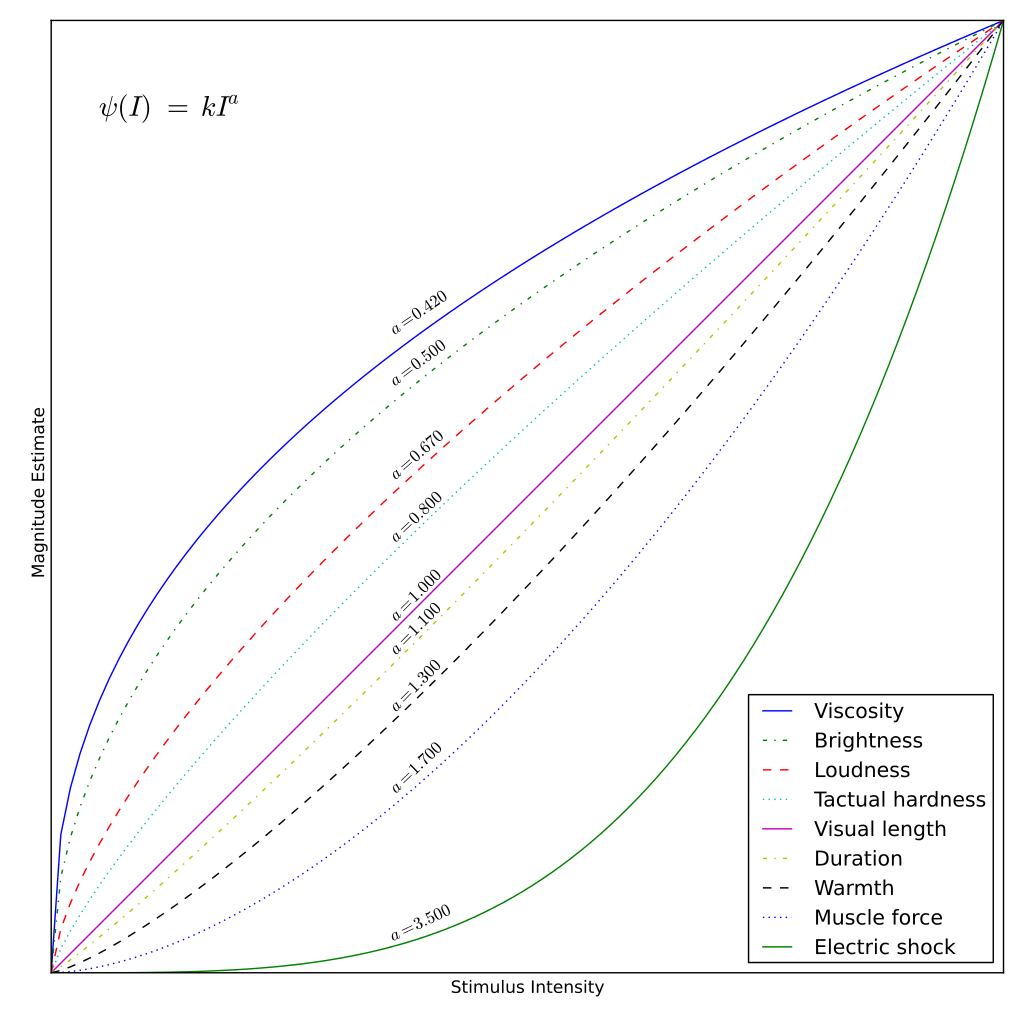
\includegraphics[width=\linewidth,height=\textheight,keepaspectratio]{Steven's_Power_Law}
    \label{fig:StevensPowerLaw}
\end{figure}
When a stimulus intensity \textit{I} is above its absolute threshold, humans perceive its magnitude as \begin{math}\Psi(I)\end{math}(perceptual strength). The exponent (dependent on stimulation freq) determines the growth rate of the perceived magnitude and ranges from 0.35 to 0.86 for vibrotactiles. Perceived intensity is a function of frequency and amplitude of vibration (also affecting perceived pitch).
    \item \emph{How good are users at judging timing of vibrotactile cues?}
Tactile perception is generally considered to have high temporal acuity.
Vibrotactile temporal resolution research cites a human's ability to distinguish successive pulses with a time gap as small as 5 ms (12000 BPM). This resolution is better than vision (25ms) but slightly worse than physiological experiments into the peripheral auditory system which cites a theoretical best case scenario of approximately 2 ms \cite{fishbach2001auditory} \cite{parsons2006neurobiology}. Keep in mind that these are temporal resolutions measured with brain scans and do not necessary translate into the limits of sensorimotor response, which, according to prior research, indicates a more realistic resolution of approximately 50ms.
    \item \emph{Can Vibrotactile cues elicit any other perceptual effects?} Below 3 Hz is considered slow kinesthetic motion. Between 10-70Hz is the sensation of rough motion or fluttering and between 100-300Hz is the sensation of smooth vibration. Subjective quality of a vibrotactile stimulus can be controlled by modifying the envelope of the stimulus amplitude.
\end{enumerate}

\subsection{Vibrotactiles} \label{vibroTT}
The exploration of touch actuation led to the evaluation of available vibrotactiles. The following is a breakdown of available vibrotactiles conducted to inform design perspective.
\begin{enumerate}
    \item Linear electromagetic actuators
    \begin{itemize}
        \item solenoid:
        \begin{itemize}
            \item can leverage resonance, large output for small input
            \item force dependent on position within magnetic field
            \item influenced by device orientation relative to gravity
            \item heats up during use
        \end{itemize}
        \item voice coil:
        \begin{itemize}
            \item linear dynamics yields consistent output, relatively easy to model
            \item \textit{C2 tactor}:
            \begin{itemize}
                \item 7.6mm contactor preloaded against the skin
                \item suspension resonates at 250Hz for maximum perceptibility
            \end{itemize}
            \item \textit{Haptuator}:
            \begin{itemize}
                \item moving magnet design
                \item not meant to touch the skin
                \item optimized to render frequencies above 50Hz
            \end{itemize}
        \end{itemize}
    \end{itemize}
    \item Rotary Electromagnetic Actuators (ERM - eccentric rotating mass)
    \begin{itemize}
        \item simple, reliable, rotate continuously with a constant voltage/current applied
        \item off-center mass affixed to output shaft so that its rotation exerts large radial forces on the body of the motor
        \item couples freq and amplitude of the resulting vibration to the motors rotational speed
        \item small voltage yields weaker vibrations
        \item intrinsic spin-up time could cause delay at the start of the cue
        \item internal static friction can prevent motor from rotating when the applied voltage is very small
    \end{itemize}
    \item Nonelectromagnetic Actuators - Piezoelectric effect
    \begin{itemize}
        \item respond to inputs very quickly and can output arbitrary waveforms
        \item typically require input on the order of 100V
        \item high stiffness of skin creates a need for relatively heavy vibrotactile actuator
        \item most don't have power to move the skin without pushing off a cumbersome mechanical ground
    \end{itemize}
    \item EAP (electroactive polymer) actuators
    \begin{itemize}
        \item uses elastomers rather than ceramics
        \item can achieve larger deformations for lower drive voltages
    \end{itemize}
    \item SMA (shape memory allow) actuators
    \begin{itemize}
        \item remembers original shape
        \item mechanical properties altered in response to temp changes
        \item slow response time, large hystoresis, high energy consumption
    \end{itemize}
    \item Pneumatic systems
    \begin{itemize}
        \item compact, light
        \item require high-pressure air source
        \item struggle to output high-frequency signals
    \end{itemize}
    \item Forced impact
    \begin{itemize}
        \item TacHammer - new technology, specs unknown, hard to acquire
    \end{itemize}
\end{enumerate}

\subsubsection{Vibrotactile Constraints}
\begin{enumerate}
    \item Create consistent mechanical coupling between actuator vibrations and users skin
    \item Slight changes to such a system drastically affect a users ability to feel and comprehend the rendered signals.
    \item For fixed actuator size/activation level, magnitude of created vibrations is inversely proportional to the mass of the object.
    \item High bandwidth accelerometer can be used to measure vibration output performance \cite{ignoto2017development}.
    \item When the application involves a large object, a wearable device, and/or multiple stimulation sites, the optimal vibrotactile rendering paradigm is to vibrate one or more small zones. 
    \begin{itemize}
    \item In a tactile display application the localization accuracy of 250-Hz vibrotactile stimuli around the waist was 74\% with 12 equidistant tactile actuators (tactors), 92\% with eight tactors, and 97\% with six tactors \cite{choi2013vibrotactile}.
    \end{itemize}
\end{enumerate}

\section{Design requirements} \label{designReq}

The initial requirement set forth by Professor Neely in the Haptic Enviro-Sensing Metronome (HESM) design draft is centered around an analogue wave that could squeeze and release. As the analogue wave approaches its crest it provides insight forecasting the approaching \textit{crusis}, allowing the user to prepare for and rebound from the "click-moment" with rich entrainment. 

This observation is in direct parallel to external vibrotactile metronome research as discussed in \ref{vibrotactileMetronome}. The constraint was such that the pulses should feel continuous and not discrete in order to capture the essence of pendulum motion.

As the intention is to encourage entrainment of the human body to external forces, the frequencies
required are quite low, based on the tempi of slow walking to running gaits
(40 bpm/.67 Hz to 180 bpm/3 Hz).

\section{Initial Prototypes} \label{initProto}
In order to capture the sensation defined in the design requirements, a series of prototypes were rapidly developed.

\subsection{Solenoid bracelet}
Initial introspection towards capturing the squeeze and release sensation led to the rapid prototyping of a simple solenoid bracelet. 
\subsubsection{Parts List}
\begin{enumerate}
    \item Adafruit Pro Trinket 5V 16MHz
    \item N-channel MOSFET
    \item 1N4004 diode
    \item mini push-pull solenoid
\end{enumerate}
\subsubsection{Assembly}
The design was inspired and assembled per \textit{Adafruit} specification \cite{Solenoid}. 
The base of an N-channel MOSFET was connected through a 1K resistor to a digital I/O pin on the trinket per Figure \ref{SolenoidSchematic}. The collector was connected through the solenoid and diode in parallel to Vcc running at 5V.
\begin{figure}[H]
    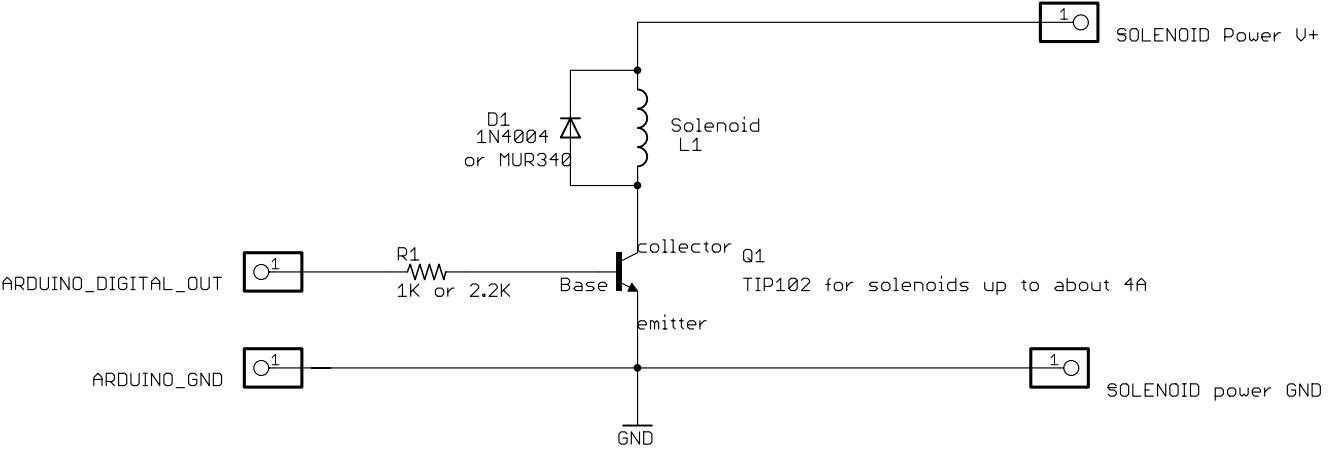
\includegraphics[width=\linewidth,height=\textheight,keepaspectratio]{Solenoid_Schematic}
    \caption{Solenoid Schematic}
    \label{SolenoidSchematic}
\end{figure}
\subsubsection{Method}
    As a voltage is applied the slug in the middle of the solenoid is pulled into the center of the coil. The actuation pulls a taught wristband attached to the chasis of the solenoid and as the voltage drops the solenoid retracts releasing tension in the wristband, shown in Figure \ref{SolenoidProto}.
    
    \begin{wrapfigure}{R}{.5\textwidth}
        \centering
        \caption{Solenoid Wristband Prototype}
        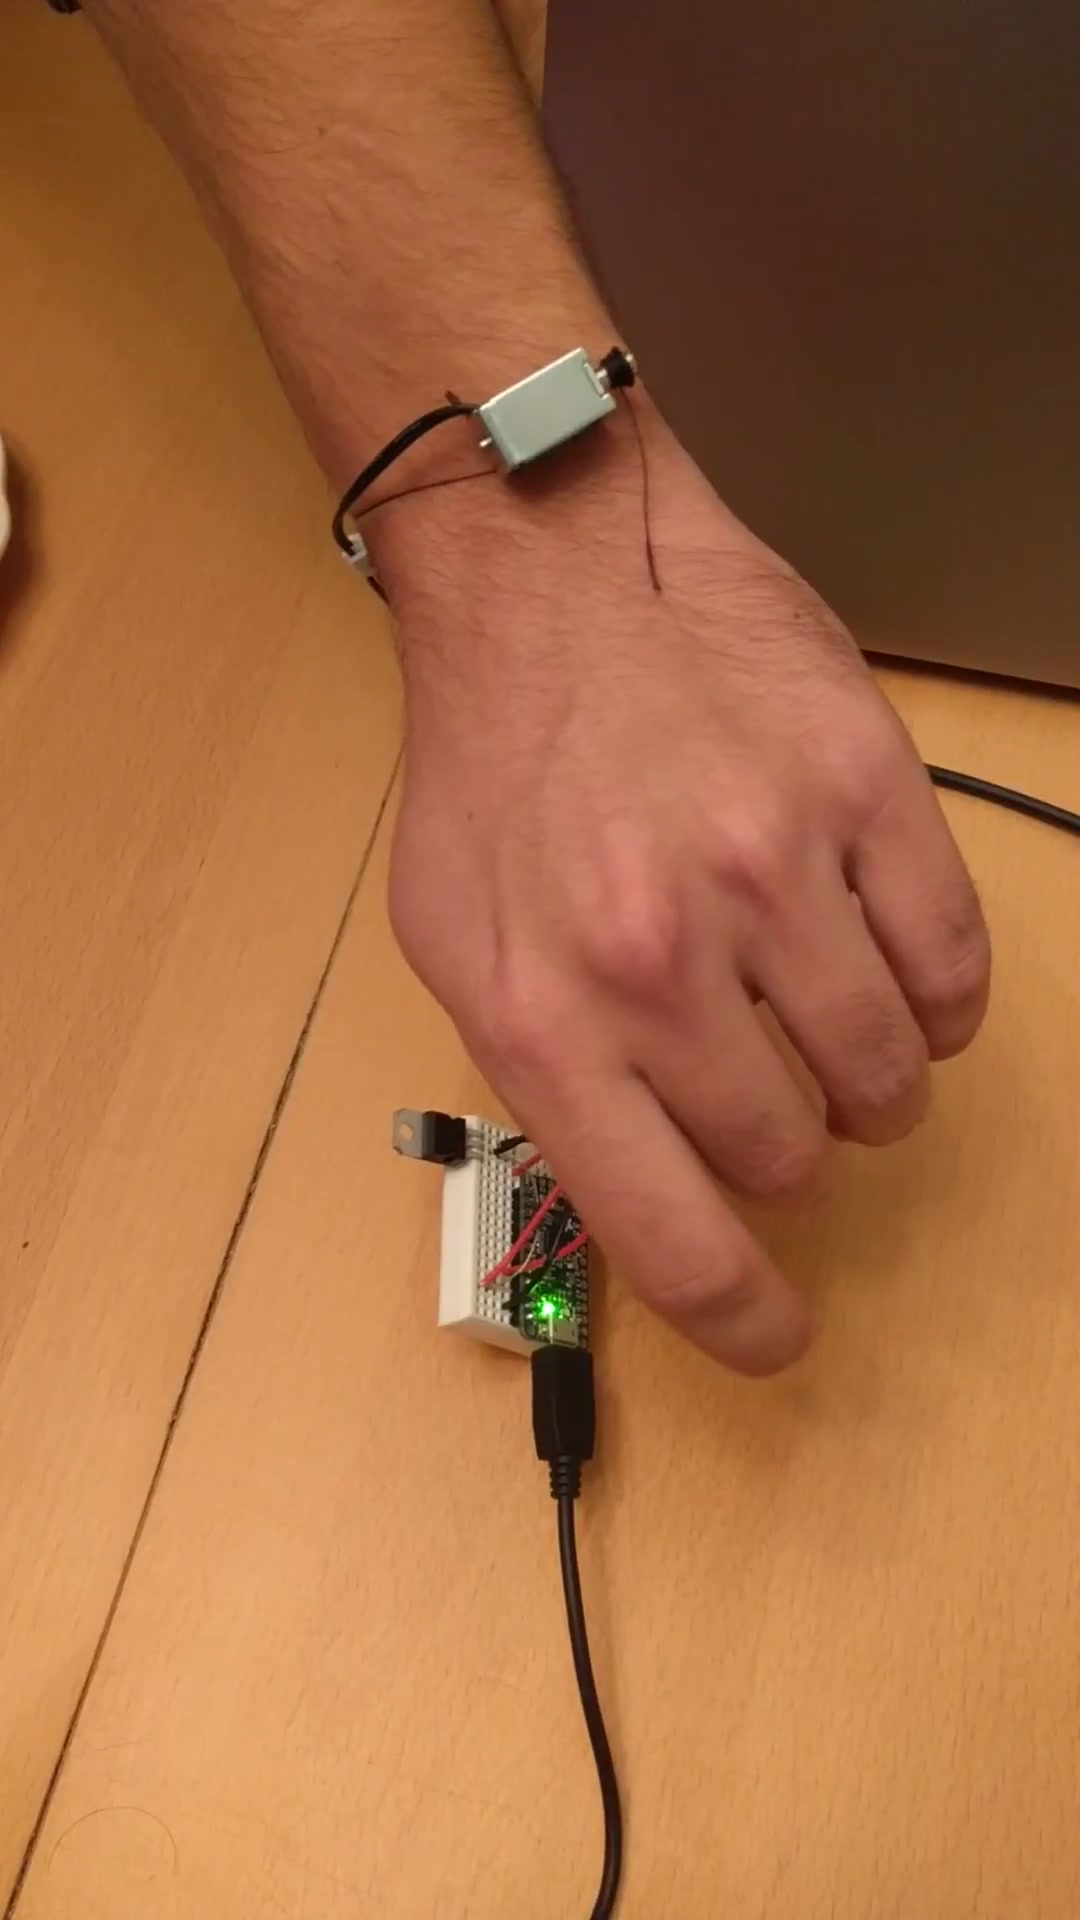
\includegraphics[width=.5\linewidth,height=.5\textheight,keepaspectratio]
        {SolenoidProto}
        \label{SolenoidProto}
    \end{wrapfigure}
    
    This was controlled in the \textit{Arduino IDE} through a simple PMW signal with increasing duty cycle which output through the digital I/O. The delay was hard coded proportional to the desired BPM.

\subsubsection{Outcome}

Due to the linear relationship between current draw and pull force, the solenoid required high current and significant voltage thus isolation from the microcontroller was ideal. The necessary rigidity of the band was a cause of discomfort and the lack of positioning options was a detriment to musicians who relied on availability of their hand. Additionally, heat dissipation was at times unsafe and unbearable since the chasis was in direct contact with the skin. Though it captured the tension and release sensation well, there seemed to be a lack of clarity with regards to communication of whether each push pull iteration was a beat length or if a single contraction was the downbeat (i.e. eighth note pulse rather than quarter note). Coupled with the bulky nature of the solenoid chasis, high power requirements and excessive heat dissipation, the solenoid prototype was quickly abandoned.
\subsection{Single vibrotactile}

The subsequent prototype iteration was the first involving a vibrotactile motor. Since the goal was to run everything off of a single board, the voltage constraint was limited to the 5V maximum per \textit{Adafruit Pro Trinket} spec. An ERM motor was chosen for its working voltage range of 2-5V and minimal coin cell form factor (10mm diameter). Like the solenoid, higher applied voltage yielded more current draw but stronger vibration. At 5V, a single motor draws 100mA. The specification was 1100 at 5V which roughly translates to 183Hz. Though not quite at the ideal 250Hz range optimal for skin sensitivity, this was deemed close enough.

To realize the spectrum of capability for vibrotactile sensation (beyond pulse width modulation of the signal) a haptic motor controller with a pre-installed library of effects was acquired. 

The goal of this design was to test the ERM sensation on a portable wearable. The MCU was altered from the Pro Trinket to the Flora which ran at 3.3V and had less digital I/O pins, but supported external connectivity and took up less surface area.

\subsubsection{Parts List}
\begin{enumerate}
    \item Vibrating mini motor disc
    \item Adafruit DRV2605L Haptic Motor Controller
    \item Flora Wearable Bluefruit LE Module
    \item Flora Wearable electronic platform
    \item LiPo Battery - 3.7v 1100mAh
\end{enumerate}
\subsubsection{Assembly}
    First, the ERM leads were soldered to the DRV2605 haptic motor controller and connected via I2C protocol to the complimentary pins on the Flora (SCL,SDA).
    To experiment with triggering the vibrotactile wirelesssly, the bluetooth low energy (BLE) module was added and the send and receive (Tx/Rx) pins were connected as referenced in Figure \ref{fig:Proto2}. The battery was connected via the built-in terminal clip and last the entire prototype was fitted into the space of a sports wristband with the vibrotactile on the inside touching the skin.

    \begin{figure}[H]
        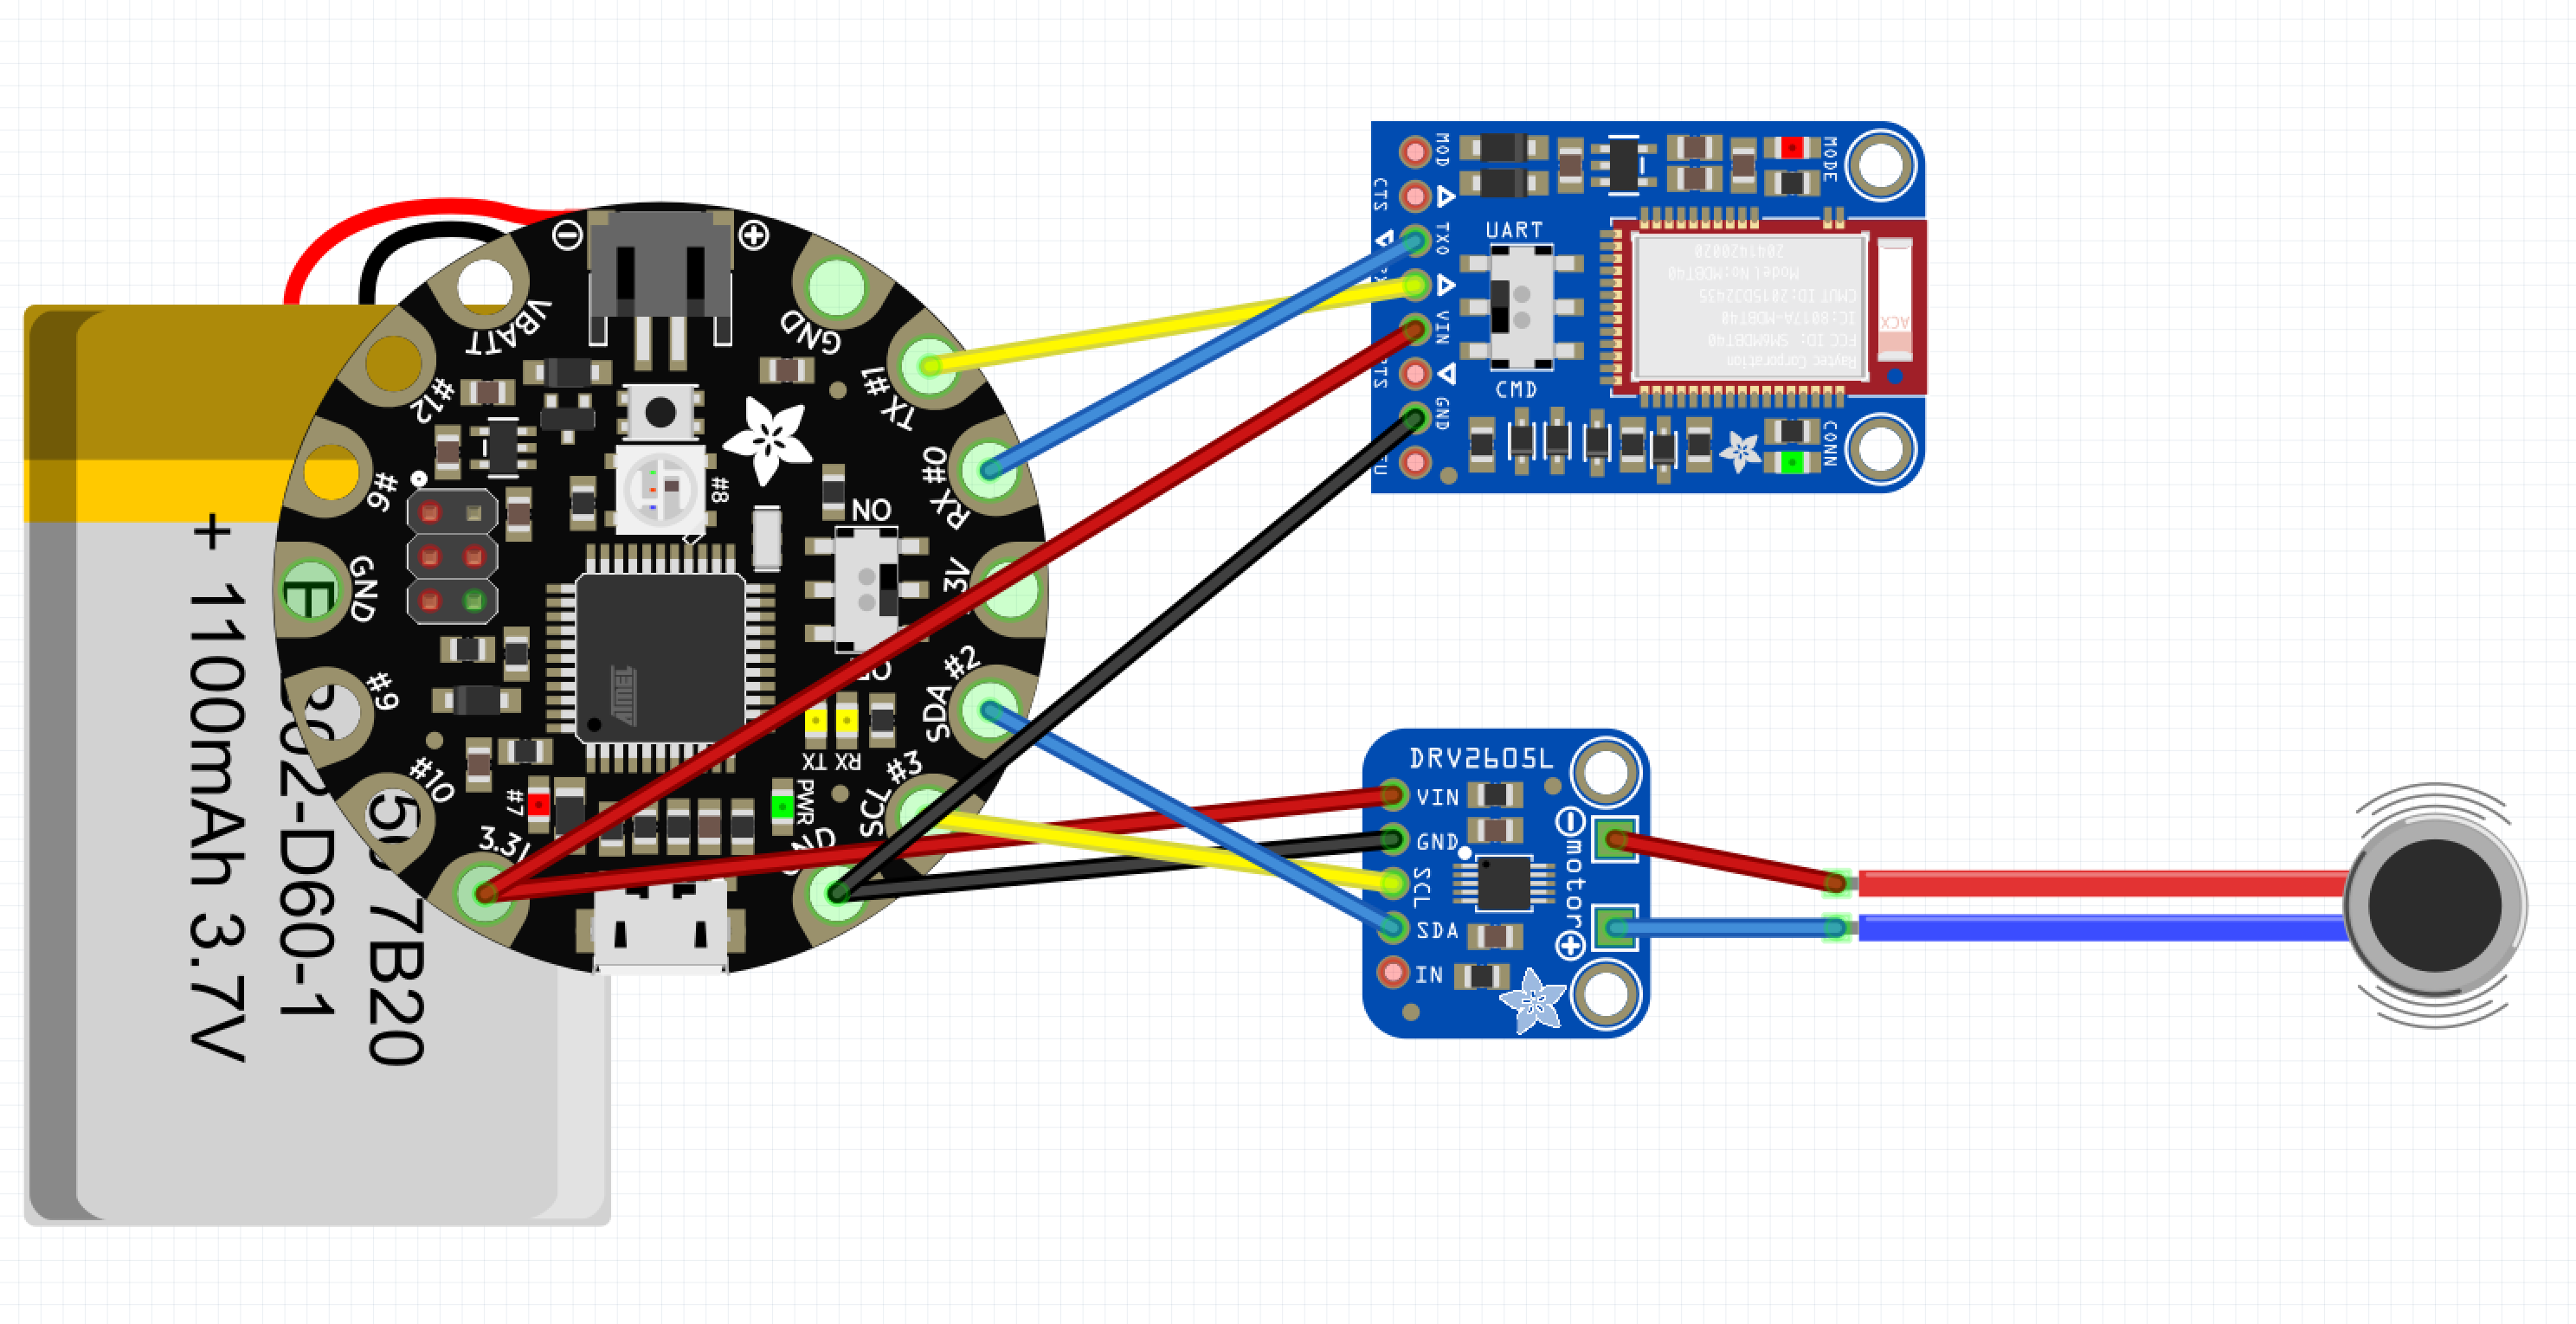
\includegraphics[width=\linewidth,height=\textheight,keepaspectratio]{Proto2_bb}
        \caption{Prototype 2 - Single vibrotactile, wireless connectivity}
        \label{fig:Proto2}
    \end{figure}

\subsubsection{Method}
    Once the hardware was setup, the haptic library was iterated through for selection of the most influential effect. The optimal sensation chosen was a queue of two chained effects according to the \underline{DRV2605 datasheet}\cite{Adafruit}:
    \begin{itemize}
        \item 83 - Transition Ramp Up Long Smooth 2 - 0 to 100\%
        \item 71 - Transition Ramp Down Long Smooth 2 - 100\% to 0
    \end{itemize}

    Within the Arduino IDE the Bluefruit library and dependencies were imported and the bluetooth low energy connection configured via UART. On the client side, the connectivity was validated via the publicly available Bluefruit application on an external Android device. The app would send integer values representing the desired BPM to the connected haptic wearable. The code was written such that upon setup and BT pairing, the main loop was polling for packets. Once received in the buffer, the new bpm value was parsed into a period value in milliseconds via equation \ref{eq:period}

    \begin{equation}
        \label{eq:period}
        period = \frac{60,000}{bpm}
    \end{equation}

    Since the highest operational bpm specified was 180, the shortest period would be an interval of 333.33 ms. This value divided in half gave the maximum allowed ramp up time for the motor, approximately 150ms. The new period value was fed into a state machine which set the on and off state of the motor based on a timer from half the calculated period as well as the 150ms off state.

    \subsubsection{Outcome}
    The singular ERM prototype granted key insight into the capability of a vibrotactile to create the desired awareness and fill the interstitial space; though it was found to be lacking the ability to fully command the wearer's attention. This was primarily due to the fact that it was driven by a 3.3V board which inhibited the vibrational strength. The next iteration needed to operate at higher voltage to get a stronger vibration. It was also deemed necessary to increase the number of vibrotactiles to work in an array format in complete synchronicity to explicitly communicate the necessary ramp down and up sensation. 
    
    Though the haptic motor controller was a critical evaluation tool for selecting the vibration effect, it was crucial for the final prototype to be able to turn on the motors at full voltage as quick as possible in order to minimize ramp up time. Chaining the motors would also optimize ramp up time in allowing a motor the time to fully spin back down while the adjacent was spinning up.

    Furthermore, the \textit{delay()} function added in the BLE section of code was causing the haptic to drift slightly in tempo beyond five minutes of runtime due to the programmatic halting and resumption of dependent timers. The next prototype would have to move away from the delay function which halted program execution.

\section{Vibrotactile Haptic Array} \label{vibroProto}
The final prototype was an array of four vibrotactiles. Several hardware advancements were implemented in order to solve design challenges. The overall process is detailed below.
\subsection{Hardware}
The main board was reverted back to that used in the solenoid prototype, the 5V 16MHz \textit{Adafruit Pro Trinket}, in order to provide maximum possible voltage to the motors. This board did not have built in serial communication so an FTDI to USB cable was necessary in order to communicate with the device. Bluetooth connectivity was abandoned to concentrate focus on minimized latency. 
\subsubsection{Parts List}
\begin{table}[H]
    \centering
    \resizebox{\columnwidth}{!}{%
    \begin{tabular}{lll}
    Part Type & Properties & Quantity \\ \hline
    Electrolytic Capacitor & capacitance 68µF; package 0405 {[}SMD, electrolytic{]}; voltage 16V & 1 \\
    Electrolytic Capacitor & capacitance 10µF; package 200 mil {[}THT, electrolytic{]}; voltage 25V & 4 \\
    Ceramic Capacitor & capacitance 100nF; package 100 mil {[}THT, multilayer{]}; voltage 6.3V & 1 \\
    Diode & package diode-1n4001; variant pth & 4 \\
    Vibration Motor & vibration motor 11000 RPM 5VDC & 4 \\
    Adafruit Pro Trinket 5V 16MHz & variant variant 1; part \# Adafruit \#2000 & 1 \\
    2N7000 FET N-Channel & package TO92; type n-channel; part \# 2N7000 & 4 \\
    220Ω Resistor & tolerance ±5\%; package 0805 {[}SMD{]}; resistance 220Ω & 5 \\
    10kΩ Resistor & tolerance ±5\%; package 0603 {[}SMD{]}; resistance 10kΩ & 1 \\
    FTDI to USB & Adafruit FTDI Serial TTL­232 USB Cable {[}ADA70{]} & 1 \\
    Shrink wrap & Heat Shrink Pack & 1
    \end{tabular}%
    }
    \caption{Vibrotactile Haptic Array Parts List}
    \label{Vibrotactile Haptic Array Parts List}
\end{table}

\subsubsection{Assembly}
Since each digital I/O of the Trinket could only source 20mA, four N-channel 2N7000 transistors were chosen to act as switches and current isolators for controlling power to the motors. These are labelled (N) in Figure \ref{FinalProto}

Each motor was connected from the power source (5V Vcc), to the drain of the transistor. When the transistor received a signal past its bias voltage of 0.8V it was switched on. This allowed the drain-source channel to be opened and an onrush of current to flow from Vcc to the motors and through to ground. 

A 1N4001 diode was placed in parallel with the motor from the 5V Vcc node to the drain of the N-channel 2N7000 to protect the transistor by shorting out the onrush of back current emitted from the motor during immediate shutoff. Principally, the motor will act as an inductor; a sudden change in current creates an equivalent voltage to keep that current flowing short term. This could fry the transistor if the diode was not in place to short out this negative voltage spike as shown in \ref{fig:MotorRinging} 
\begin{figure}[H]
    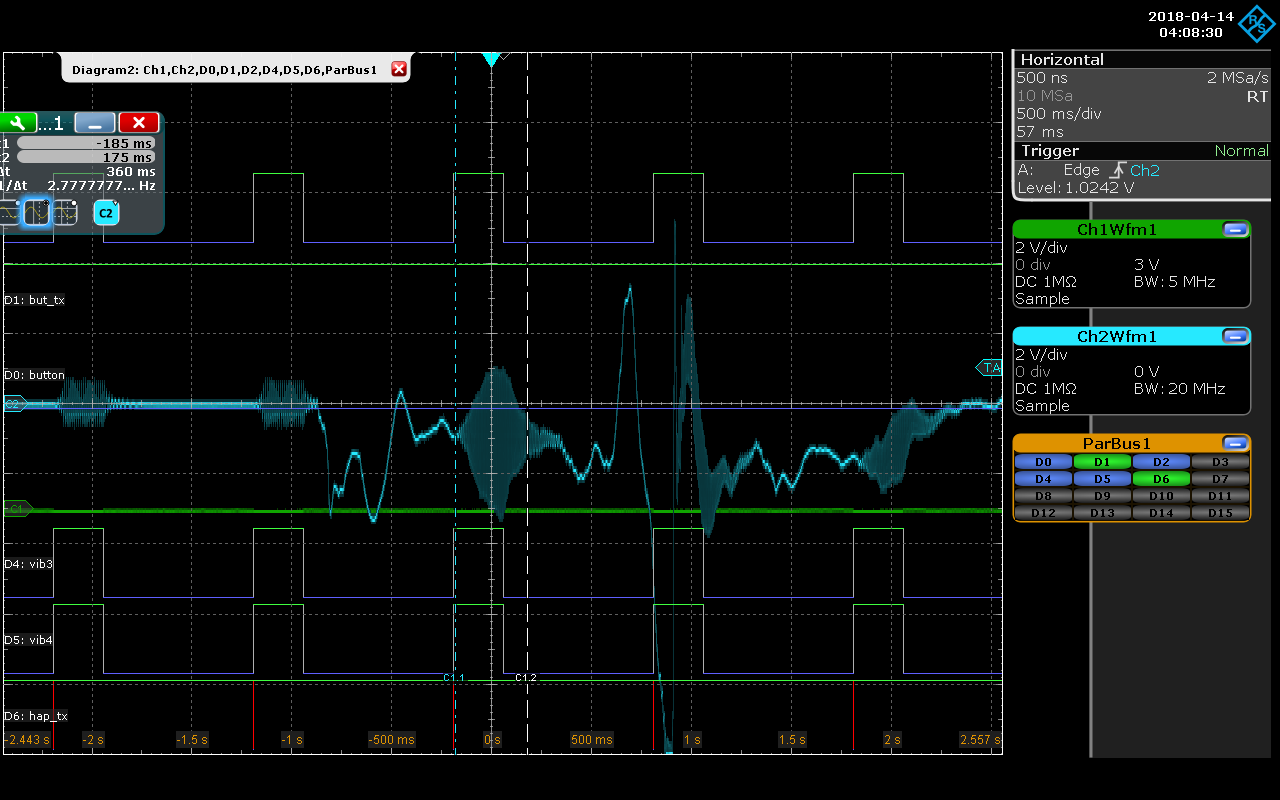
\includegraphics[width=\linewidth,height=\textheight,keepaspectratio]
    {ringing}
    \caption{Motor ringing after abrupt shutoff}
    \label{fig:MotorRinging}
\end{figure}

The digital pins 5,6,9,10 (denoted with yellow and grey wires in Figure \ref{fig:FinalProto}) output a pulse-width modulated signal to be used as triggers, or control switches, for the transistors. In order to limit the current that the digital output must source and to protect the transistor gate, a 220 Ohm resistor was connected across the digital I/O pin and the gate of the 2N7000 for each pin.

\begin{figure}[H]
    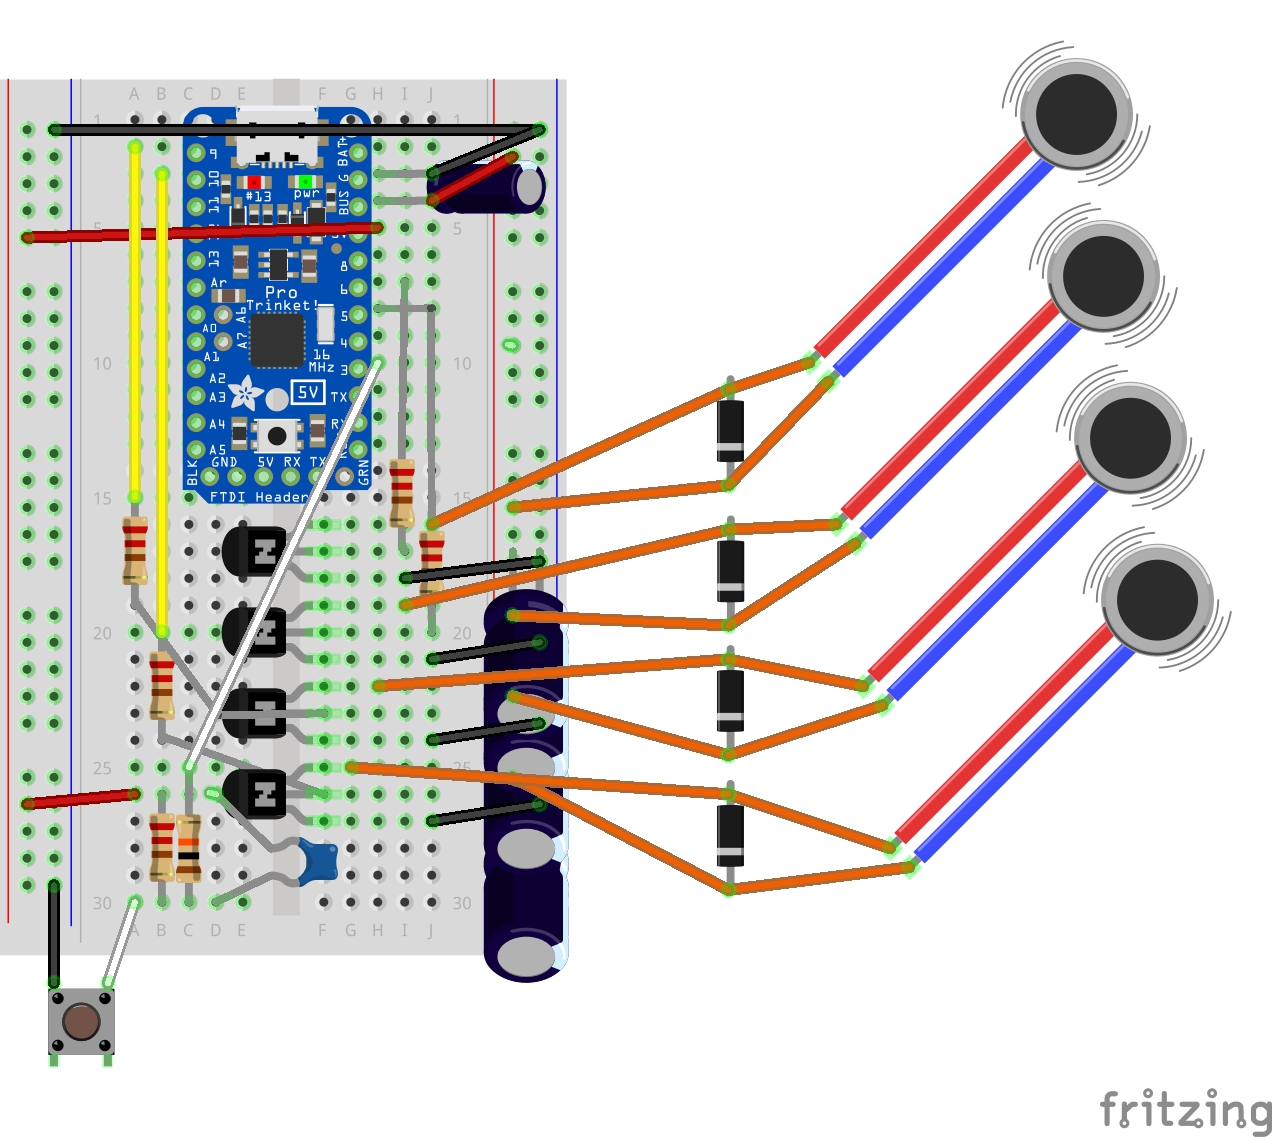
\includegraphics[width=\linewidth,height=\textheight,keepaspectratio]
    {FinalProto_bb}
    \caption{Final prototype wiring mockup}
    \label{fig:FinalProto}
\end{figure}

The voltage across the rails (Vcc and ground) was viewed on a Rohde \& Schwarz RTO 2004 oscilloscope. The analyzed waveform showed some unfavorable dips primarily when all motors were running due to the high current draw from the ERMs in addition to some ringing (overshoot), seen in Fig \ref{fig:precaps}.
\begin{figure}[H]
    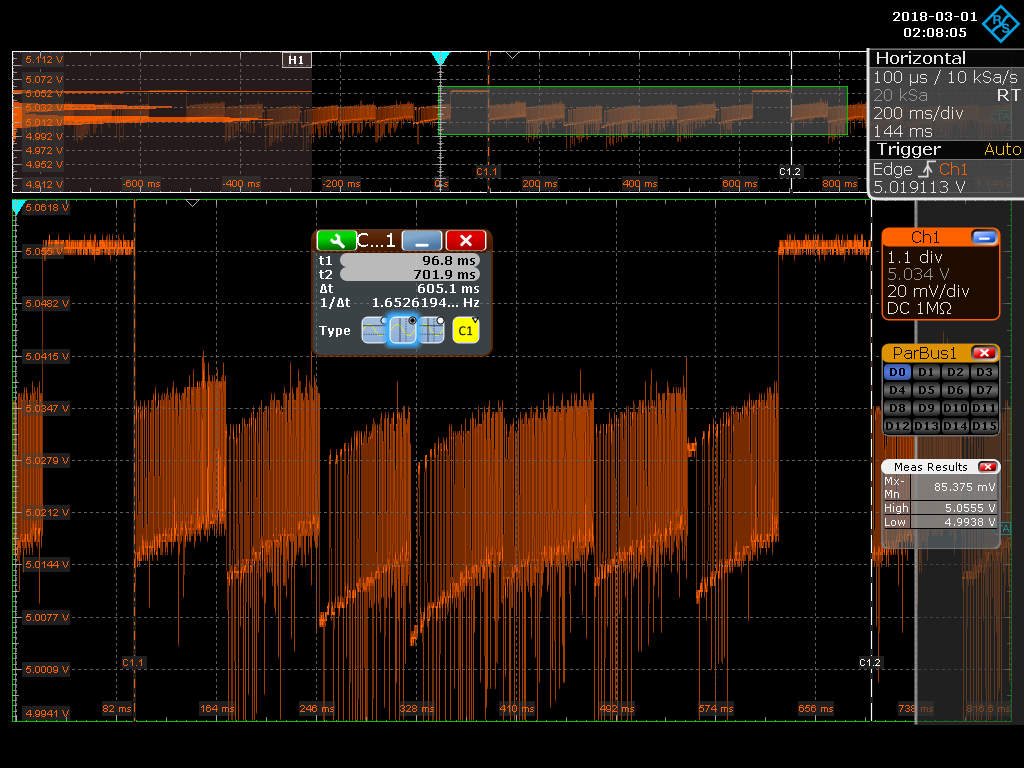
\includegraphics[width=\linewidth,height=\textheight,keepaspectratio]
    {pre-cap}
    \caption{V drop across Vcc and HF ringing: Pre-cap}
    \label{fig:precaps}
\end{figure}
\subsection{Improvements}
Capacitors were added to act as buffers from the power source to the motors, in doing so they helped provide immediate current to the motors when the PWM input signal engaged the transistor and the motor would go from an off state to an immediate on state drawing high amounts of current. Large electrolytic capacitors are known for their ability to supply high currents for a few milliseconds, more so than a battery or in the haptic wearables case, USB power. These were added across Vcc and ground nearest to the Trinket as well as across each of the node rails nearest to the motors. The change in output shape can be analyzed in Fig \ref{fig:postcaps}.

\begin{figure}[H]
    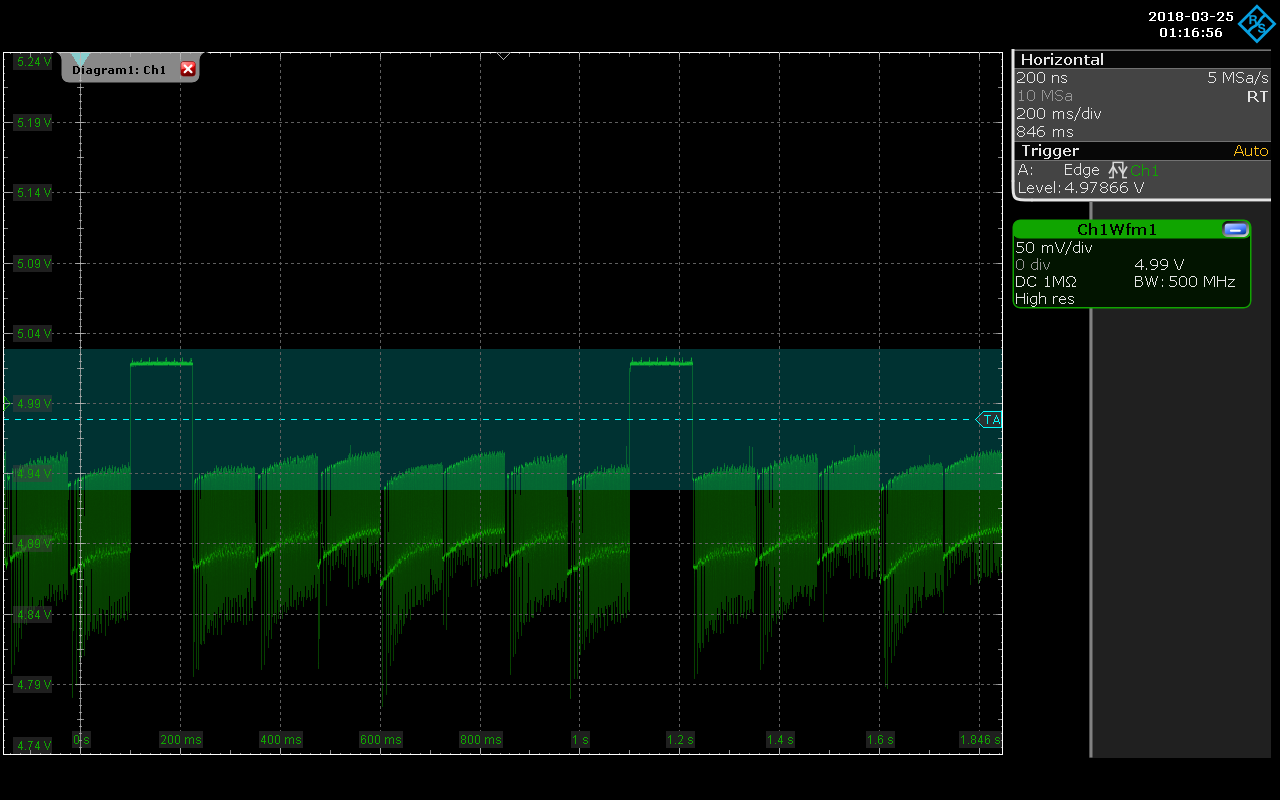
\includegraphics[width=\linewidth,height=\textheight,keepaspectratio]
    {post-cap}
    \caption{V drop across Vcc: Post-cap}
    \label{fig:postcaps}
\end{figure}

As an additional manual tap tempo option for the user to experiment with, a push-button was added and connected to the only interrupt capable pin on the Trinket, PIN 3. An RC combination was chosen to act as a low-pass filter to protect against debounce scenarios.

\begin{figure}[H]
    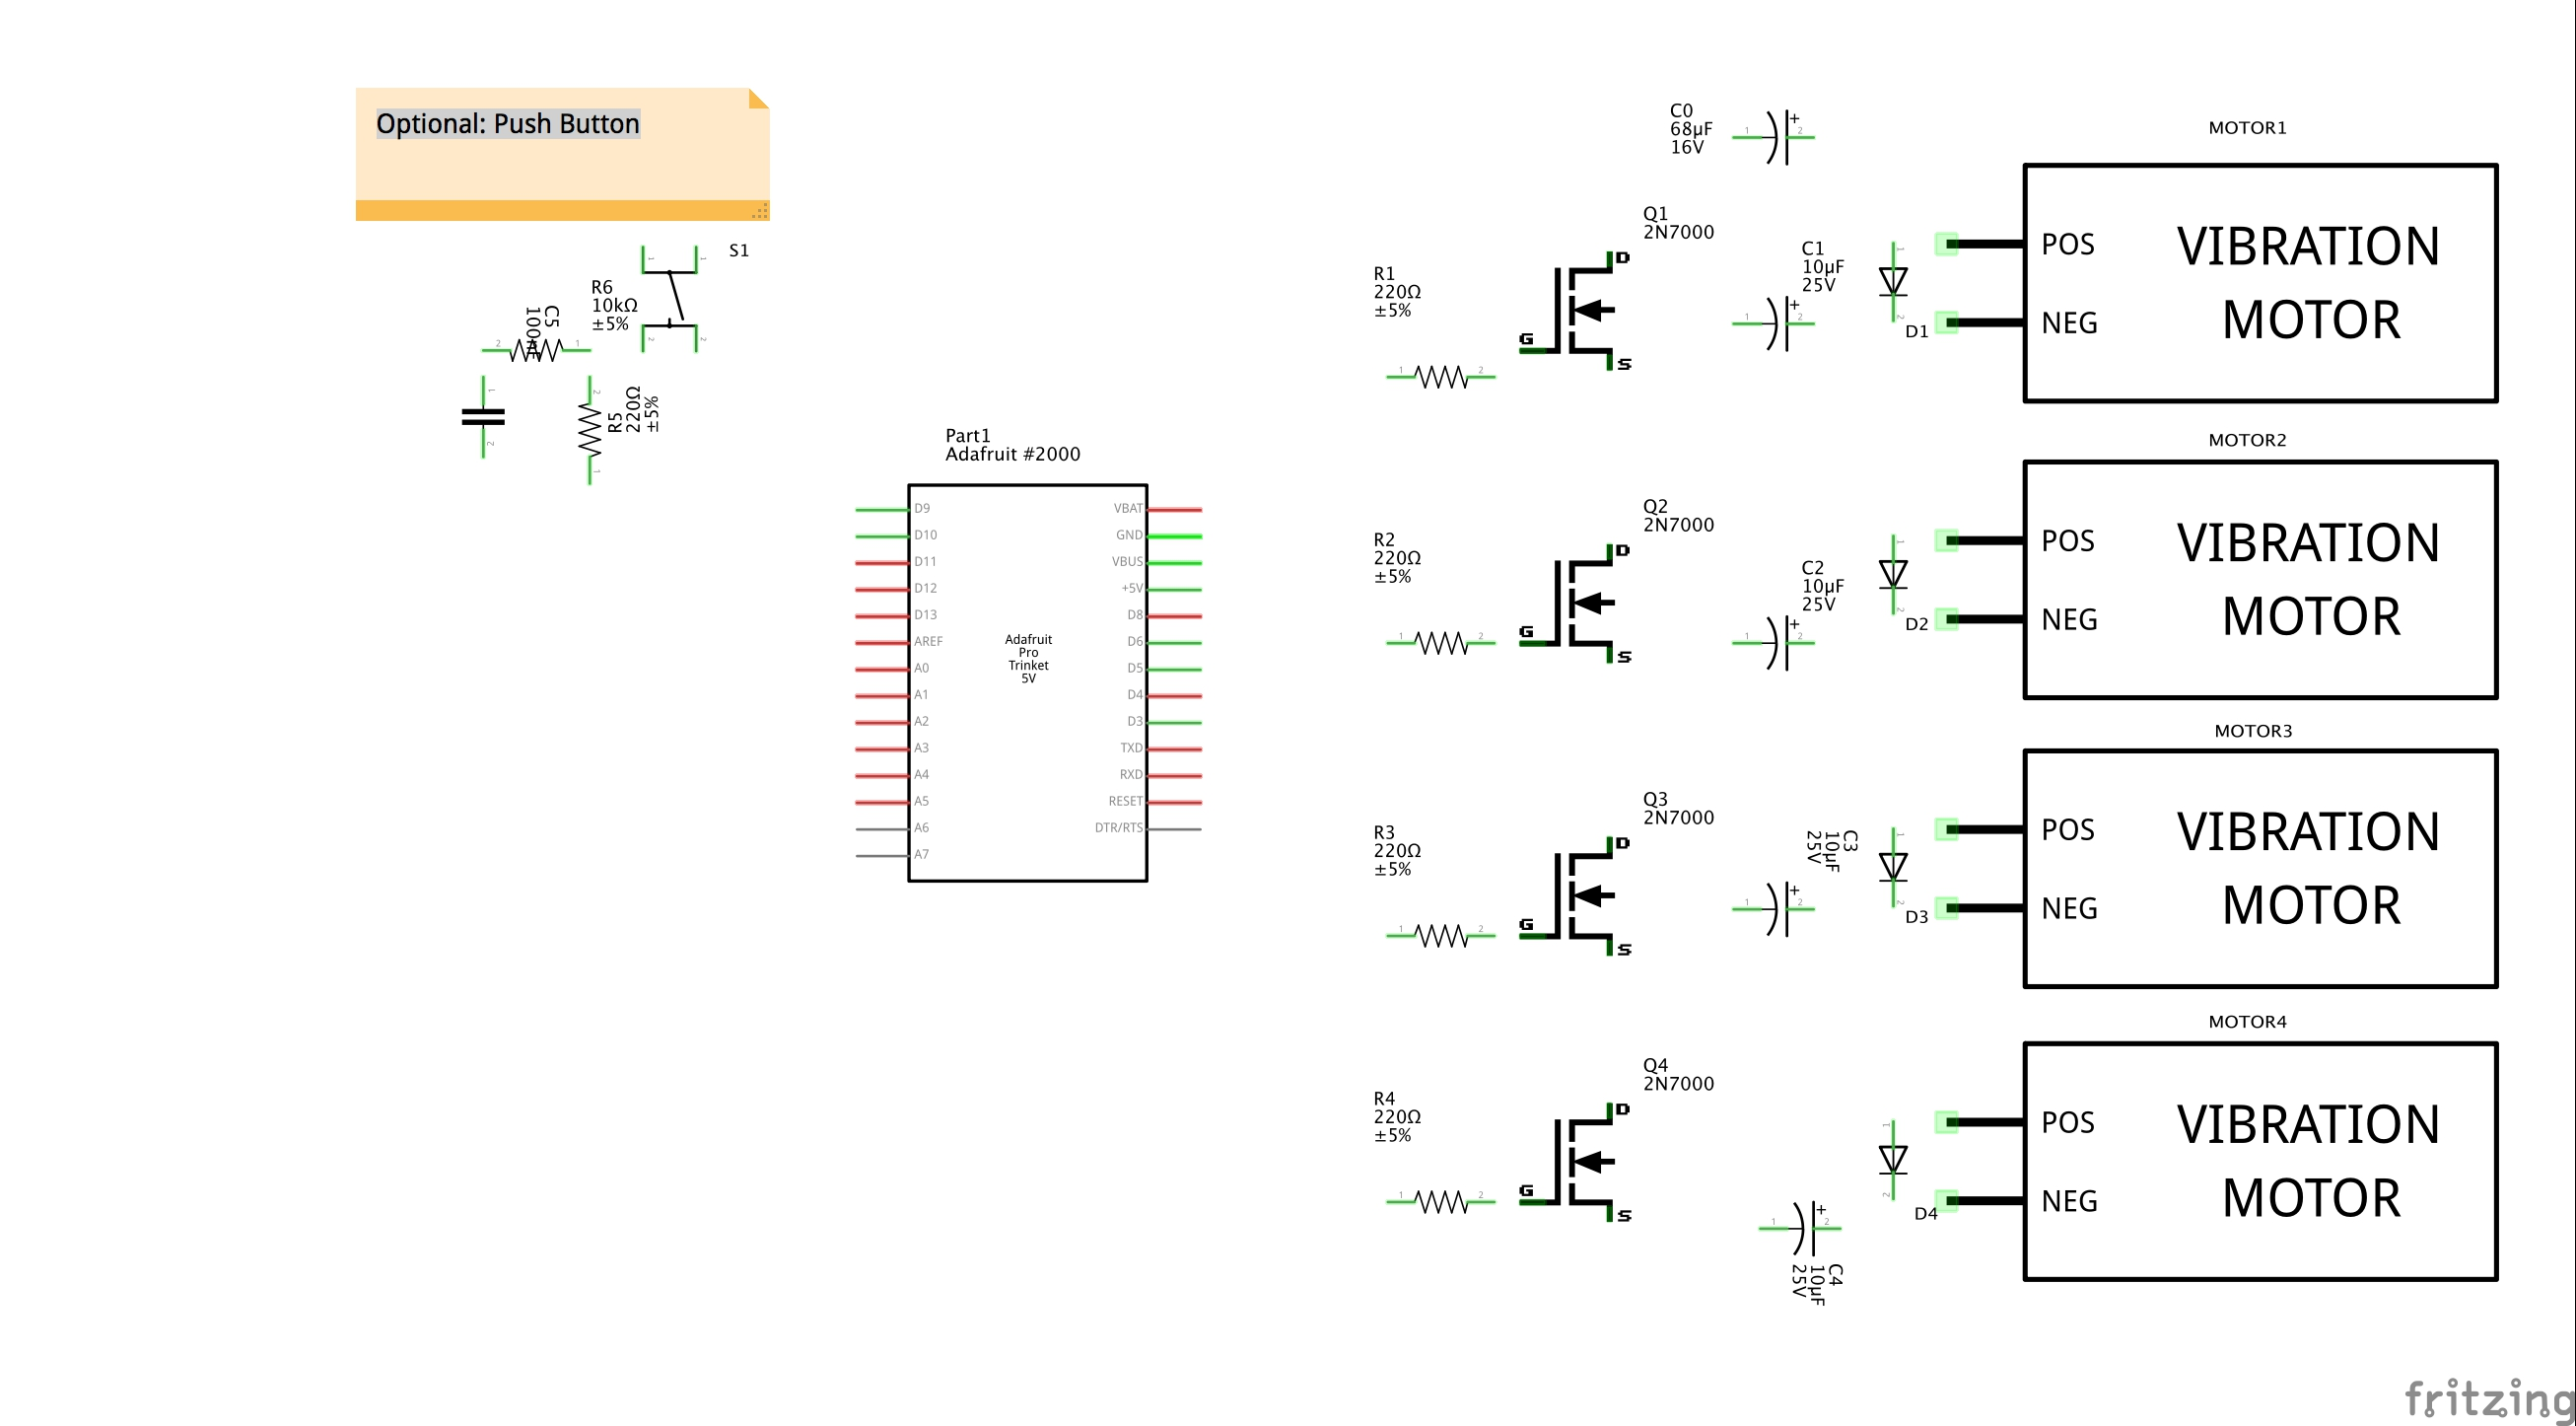
\includegraphics[width=\textwidth,height=\textheight,keepaspectratio]
    {FinalProto_schem}
    \caption{Final prototype abstracted schematic}
    \label{fig:FinalProtoSchem}
\end{figure}

\subsubsection{Motor Characterization}
In order to determine an accurate baseline for motor ramp up, a singular motor was firmly attached to a piezoelectric transducer. The remaining motors were connected to the digital bus of the scope for timing analysis. 
\begin{figure}[H]
    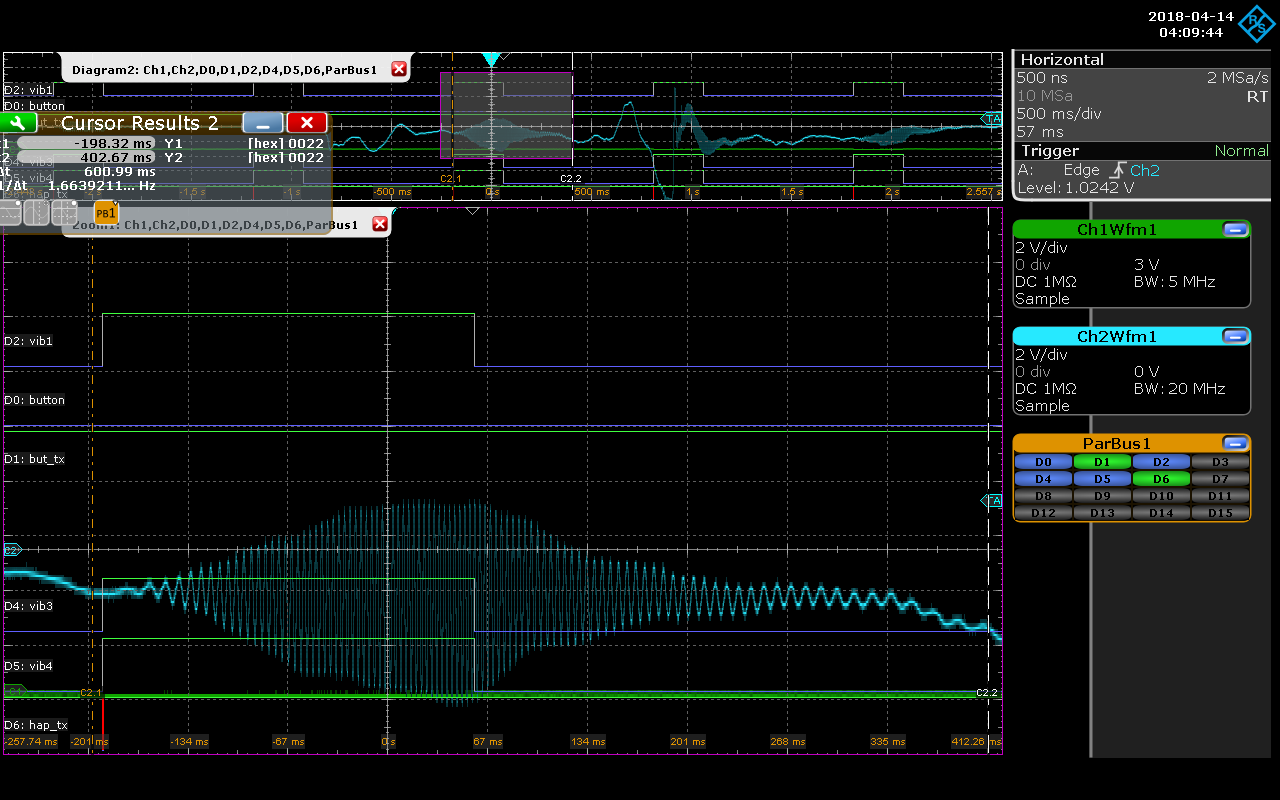
\includegraphics[width=\textwidth,height=\textheight,keepaspectratio]
    {motorramp}
    \caption{Motor ramp up time}
    \label{fig:MotorRampUp}
\end{figure}

As seen in Fig \ref{fig:MotorRampUp}, the motors reach full amplitude over approximately 67ms before the signal goes low and starts to decay. The AC shape of the waveform is due to the nature of the ERM. The rotating mass translates left and right movement into a voltage oscillating in amplitude. Multiple ramp up times were averaged using this method such that the time before perceptibility was determined to be about a quarter of the ramp up time (approximately $50ms$), in agreement with \ref{HD}. This is clearly shown in Fig \ref{fig:MotorRampUp2} below.
\begin{figure}[H]
    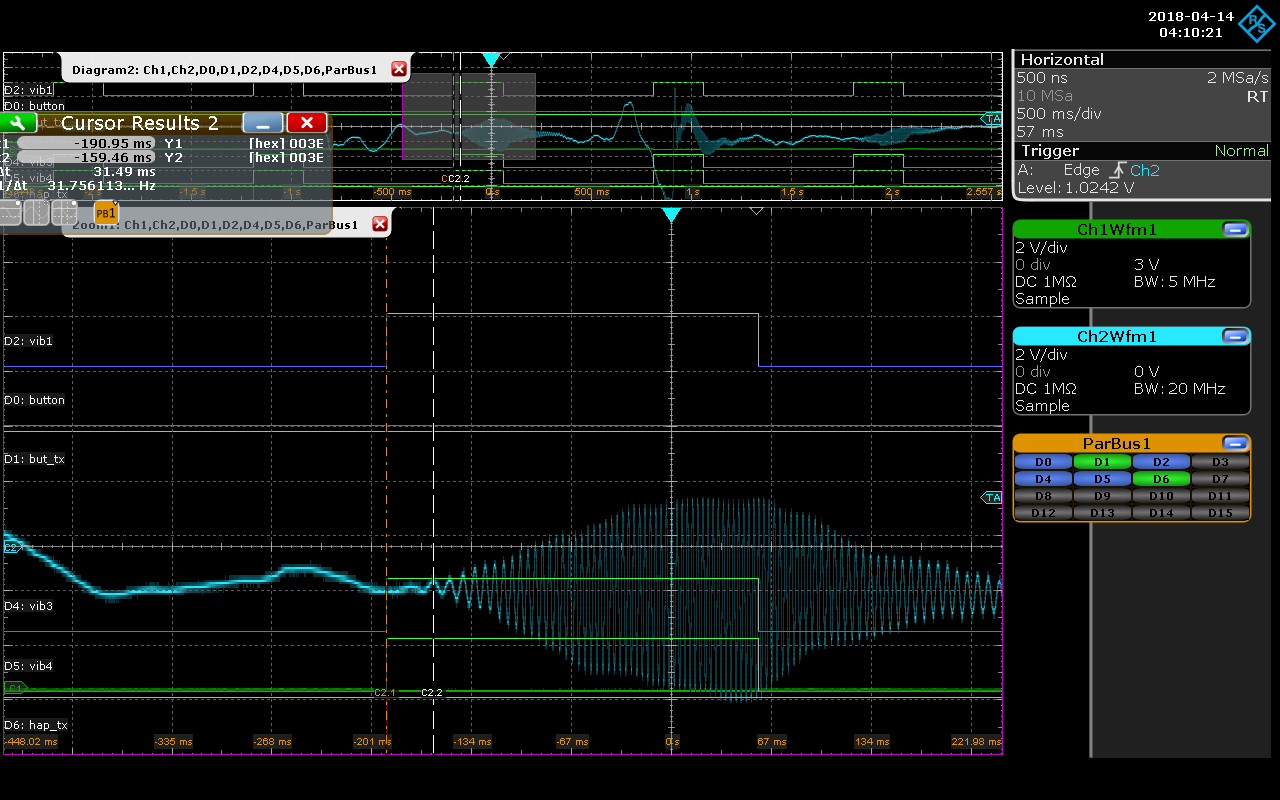
\includegraphics[width=\textwidth,height=\textheight,keepaspectratio]
    {motorramp2}
    \caption{$50ms$ motor ramp up time to perceptibility}
    \label{fig:MotorRampUp2}
\end{figure}

\subsection{Software}
The code was written in the Arduino IDE which utilizes C++. Outside of the tap tempo hardware push button, the main control flow was through serial communication over FTDI. The device communicated at 115200 baud and a small method was written to read the serial buffer and parse the incoming bytes into integers. The first input was a setter to store the current operation mode with 1 being the Discrete (Instantaneous) Mode and 2 Continuous. Afterwards, any other number (thresholded from 20 to 220) would be stored as the bpm. The period was calculated using formula \ref{eq:period}

The main control flow was two state machines which were delay independent. Depending on mode selection it would send digitalWrite commands to each motor within the set time period.
Though the analogWrite functionality built into the Arduino IDE could PWM the signal and potentially control the motor just below its turn on state, the transistors would not allow this due to their rapid speed and turn on voltage and the motors would be always vibrating. This was a design decision informed by the previous single vibrotactile prototype implementation.

The first state started a millisecond precision timer. In discrete mode the second state wrote all digitalIO pins HIGH for a quarter of the period as shown in Fig \ref{fig:state1}. A half on/off implementation was considered but determined to be not as efficient in communicating rapid pulses since the ramp down time overlapped with the next on period. During this state a flag was printed over serial to be read in later indicating when the test software could timestamp the onset.

\begin{lstlisting}[language=C]
    void go(){
        if(discrete==true){
            switch (newState){
              case READY:
                if(start){
                  average = avg;
                  startTime=millis();
                  newState++;
                }
                break;
              case ON: 
                digitalWrite(vibPins[0],HIGH);
                digitalWrite(vibPins[1],HIGH);
                digitalWrite(vibPins[2],HIGH);
                digitalWrite(vibPins[3],HIGH);
                if((millis()-startTime) >= ((average * 1)/4)){
                  newState++;
                  Serial.println("onset");
                }
                break;
              case OFF:
                digitalWrite(vibPins[0],LOW);
                digitalWrite(vibPins[1],LOW);
                digitalWrite(vibPins[2],LOW);
                digitalWrite(vibPins[3],LOW);
                if(millis()-startTime >= average){
                  newState=0;
                }
                break;
              default:
                break;
            }
        }
\end{lstlisting}
% \caption{Discrete/Instantaneous state machine}

The state machine in continuous mode functioned similarly but was divided into 4 ramp-up states and 4 ramp-down states as shown in Fig \ref{fig:state2}. Each state held its vibrotactile high for 1/9 of the overall period or IOI but lingered on the fourth vibrotactile slightly longer \textit{(2/9th's * IOI)} to convey the pinnacle of the beat. This state also sent the onset trigger.

% \caption{Continous state machine}
\begin{lstlisting}[language=C]
    if(discrete==false){
        switch (state) {
          case START:
            if(start){
              average = avg;
              startTime=millis(); 
              state++;
            }
            break;
          case RAMPUP_STEP_1:
            digitalWrite(vibPins[0],HIGH);
            if((millis()-startTime) >= ((average * 1)/9)){
              state++;
            }
            break;
          case RAMPUP_STEP_2:
            digitalWrite(vibPins[0],LOW);
            digitalWrite(vibPins[1],HIGH);
            if((millis()-startTime) >= ((average * 2)/9)){
              state++;
            }
            break;
          case RAMPUP_STEP_3:
            digitalWrite(vibPins[1],LOW);
            digitalWrite(vibPins[2],HIGH);
            if((millis()-startTime) >= ((average * 3)/9)){
              state++;
            }
            break;
          case RAMPUP_STEP_4:
            digitalWrite(vibPins[2],LOW);
            digitalWrite(vibPins[3],HIGH);
            if((millis()-startTime) >= ((average * 5)/9)){
              state++;
              Serial.println("onset");
            }
            break;
          case RAMPDOWN_STEP_5:
            digitalWrite(vibPins[3],LOW);
            digitalWrite(vibPins[2],HIGH);
            if((millis()-startTime) >= ((average * 6)/9)){
              state++;
            }
            break;
          case RAMPDOWN_STEP_6:
            digitalWrite(vibPins[2],LOW);
            digitalWrite(vibPins[1],HIGH);
            if((millis()-startTime) >= ((average * 7)/9)){
              state++;
            }
            break;
          case RAMPDOWN_STEP_7:
            digitalWrite(vibPins[1],LOW);
             digitalWrite(vibPins[0],HIGH);
            if((millis()-startTime) >= ((average * 8)/9)){
              state++;
            }
            break;
           case END:
              digitalWrite(vibPins[0],LOW);
             if((millis()-startTime) >= average){
               state=0; 
             }
            break;
          default:
            break;
        }
      }
\end{lstlisting}

% ********************************************************************************
%                                 Back Matter
% ********************************************************************************

\backmatter

% Normal line spacing
\singlespace

% By default \bibsection is \chapter*, but we really want this to show
% up in the table of contents and pdf bookmarks.
\renewcommand{\bibsection}{\chapter{\bibname}}
% Additionally, redefine the chapter header to remove the chapter number.
\renewcommand{\chaptermark}[1]{%
  \markboth{\color{headergray}{#1}}{}
}


%\newcommand{\bibpreamble}{This text goes between the ``Bibliography''
%  header and the actual list of references}
\bibliographystyle{ieeetr}

% No whitespace allowed in the reference files list, ever.
\bibliography{bibliography/references}
\end{document}
